\documentclass[twoside]{book}

% Packages required by doxygen
\usepackage{fixltx2e}
\usepackage{calc}
\usepackage{doxygen}
\usepackage[export]{adjustbox} % also loads graphicx
\usepackage{graphicx}
\usepackage[utf8]{inputenc}
\usepackage{makeidx}
\usepackage{multicol}
\usepackage{multirow}
\PassOptionsToPackage{warn}{textcomp}
\usepackage{textcomp}
\usepackage[nointegrals]{wasysym}
\usepackage[table]{xcolor}

% NLS support packages
\usepackage[spanish]{babel}
% Font selection
\usepackage[T1]{fontenc}
\usepackage[scaled=.90]{helvet}
\usepackage{courier}
\usepackage{amssymb}
\usepackage{sectsty}
\renewcommand{\familydefault}{\sfdefault}
\allsectionsfont{%
  \fontseries{bc}\selectfont%
  \color{darkgray}%
}
\renewcommand{\DoxyLabelFont}{%
  \fontseries{bc}\selectfont%
  \color{darkgray}%
}
\newcommand{\+}{\discretionary{\mbox{\scriptsize$\hookleftarrow$}}{}{}}

% Page & text layout
\usepackage{geometry}
\geometry{%
  a4paper,%
  top=2.5cm,%
  bottom=2.5cm,%
  left=2.5cm,%
  right=2.5cm%
}
\tolerance=750
\hfuzz=15pt
\hbadness=750
\setlength{\emergencystretch}{15pt}
\setlength{\parindent}{0cm}
\setlength{\parskip}{3ex plus 2ex minus 2ex}
\makeatletter
\renewcommand{\paragraph}{%
  \@startsection{paragraph}{4}{0ex}{-1.0ex}{1.0ex}{%
    \normalfont\normalsize\bfseries\SS@parafont%
  }%
}
\renewcommand{\subparagraph}{%
  \@startsection{subparagraph}{5}{0ex}{-1.0ex}{1.0ex}{%
    \normalfont\normalsize\bfseries\SS@subparafont%
  }%
}
\makeatother

% Headers & footers
\usepackage{fancyhdr}
\pagestyle{fancyplain}
\fancyhead[LE]{\fancyplain{}{\bfseries\thepage}}
\fancyhead[CE]{\fancyplain{}{}}
\fancyhead[RE]{\fancyplain{}{\bfseries\leftmark}}
\fancyhead[LO]{\fancyplain{}{\bfseries\rightmark}}
\fancyhead[CO]{\fancyplain{}{}}
\fancyhead[RO]{\fancyplain{}{\bfseries\thepage}}
\fancyfoot[LE]{\fancyplain{}{}}
\fancyfoot[CE]{\fancyplain{}{}}
\fancyfoot[RE]{\fancyplain{}{\bfseries\scriptsize Generado por Doxygen }}
\fancyfoot[LO]{\fancyplain{}{\bfseries\scriptsize Generado por Doxygen }}
\fancyfoot[CO]{\fancyplain{}{}}
\fancyfoot[RO]{\fancyplain{}{}}
\renewcommand{\footrulewidth}{0.4pt}
\renewcommand{\chaptermark}[1]{%
  \markboth{#1}{}%
}
\renewcommand{\sectionmark}[1]{%
  \markright{\thesection\ #1}%
}

% Indices & bibliography
\usepackage{natbib}
\usepackage[titles]{tocloft}
\setcounter{tocdepth}{3}
\setcounter{secnumdepth}{5}
\makeindex

% Hyperlinks (required, but should be loaded last)
\usepackage{ifpdf}
\ifpdf
  \usepackage[pdftex,pagebackref=true]{hyperref}
\else
  \usepackage[ps2pdf,pagebackref=true]{hyperref}
\fi
\hypersetup{%
  colorlinks=true,%
  linkcolor=blue,%
  citecolor=blue,%
  unicode%
}

% Custom commands
\newcommand{\clearemptydoublepage}{%
  \newpage{\pagestyle{empty}\cleardoublepage}%
}

\usepackage{caption}
\captionsetup{labelsep=space,justification=centering,font={bf},singlelinecheck=off,skip=4pt,position=top}

%===== C O N T E N T S =====

\begin{document}

% Titlepage & ToC
\hypersetup{pageanchor=false,
             bookmarksnumbered=true,
             pdfencoding=unicode
            }
\pagenumbering{alph}
\begin{titlepage}
\vspace*{7cm}
\begin{center}%
{\Large Práctica de P\+R\+O2\+: Evolución de las especies. \\[1ex]\large P\+E\+I\+L\+IN NI }\\
\vspace*{1cm}
{\large Generado por Doxygen 1.8.13}\\
\end{center}
\end{titlepage}
\clearemptydoublepage
\pagenumbering{roman}
\tableofcontents
\clearemptydoublepage
\pagenumbering{arabic}
\hypersetup{pageanchor=true}

%--- Begin generated contents ---
\chapter{Página principal}
\label{index}\hypertarget{index}{}Evolución de Especies.

Programa principal que simula la evolución de las especies según lo similares que sean. El usuario tiene una lista de comandos disponibles que le permite seleccionar diversas operaciones. El programa contiene múltiples módulos donde están implementadas esas funciones que llevan a cabo las operaciones requeridas. Cada uno contiene sus funciones que permiten modificar el conjunto siempre que el usuario lo requiera sea añadiendo o eliminando una o un conjunto de especies o calculando sus respectivas distancias. 
\chapter{Índice de clases}
\section{Lista de clases}
Lista de las clases, estructuras, uniones e interfaces con una breve descripción\+:\begin{DoxyCompactList}
\item\contentsline{section}{\hyperlink{class_cjt___clusters}{Cjt\+\_\+\+Clusters} \\*Representa el ciclo evolutivo de los clusters según la diferencia de distancias entre estos }{\pageref{class_cjt___clusters}}{}
\item\contentsline{section}{\hyperlink{class_cjt___especies}{Cjt\+\_\+\+Especies} \\*Representa la agrupación de las especies y una serie de operaciones para formar este conjunto }{\pageref{class_cjt___especies}}{}
\item\contentsline{section}{\hyperlink{class_cluster}{Cluster} \\*Representa el conjunto de características y operaciones de los clústers }{\pageref{class_cluster}}{}
\item\contentsline{section}{\hyperlink{class_especie}{Especie} \\*Representa el conjunto de características y operaciones de las especies }{\pageref{class_especie}}{}
\end{DoxyCompactList}

\chapter{Indice de archivos}
\section{Lista de archivos}
Lista de todos los archivos con descripciones breves\+:\begin{DoxyCompactList}
\item\contentsline{section}{\hyperlink{_cjt___clusters_8cc}{Cjt\+\_\+\+Clusters.\+cc} \\*Implementación de la clase \hyperlink{class_cjt___clusters}{Cjt\+\_\+\+Clusters} }{\pageref{_cjt___clusters_8cc}}{}
\item\contentsline{section}{\hyperlink{_cjt___clusters_8hh}{Cjt\+\_\+\+Clusters.\+hh} \\*Especificación \hyperlink{class_cjt___clusters}{Cjt\+\_\+\+Clusters} }{\pageref{_cjt___clusters_8hh}}{}
\item\contentsline{section}{\hyperlink{_cjt___especies_8cc}{Cjt\+\_\+\+Especies.\+cc} \\*Implementación de la clase \hyperlink{class_cjt___especies}{Cjt\+\_\+\+Especies} }{\pageref{_cjt___especies_8cc}}{}
\item\contentsline{section}{\hyperlink{_cjt___especies_8hh}{Cjt\+\_\+\+Especies.\+hh} \\*Especificación \hyperlink{class_cjt___especies}{Cjt\+\_\+\+Especies} }{\pageref{_cjt___especies_8hh}}{}
\item\contentsline{section}{\hyperlink{_cluster_8cc}{Cluster.\+cc} \\*Implementación de la clase \hyperlink{class_cluster}{Cluster} }{\pageref{_cluster_8cc}}{}
\item\contentsline{section}{\hyperlink{_cluster_8hh}{Cluster.\+hh} \\*Especificación de \hyperlink{class_cluster}{Cluster} }{\pageref{_cluster_8hh}}{}
\item\contentsline{section}{\hyperlink{_especie_8cc}{Especie.\+cc} \\*Implementación de la clase \hyperlink{class_especie}{Especie} }{\pageref{_especie_8cc}}{}
\item\contentsline{section}{\hyperlink{_especie_8hh}{Especie.\+hh} \\*Especificación de una classe \hyperlink{class_especie}{Especie} }{\pageref{_especie_8hh}}{}
\item\contentsline{section}{\hyperlink{program_8cc}{program.\+cc} \\*Programa principal para el ejercicio {\itshape Evolución de las Especies} }{\pageref{program_8cc}}{}
\end{DoxyCompactList}

\chapter{Documentación de las clases}
\hypertarget{class_cjt___clusters}{}\section{Referencia de la Clase Cjt\+\_\+\+Clusters}
\label{class_cjt___clusters}\index{Cjt\+\_\+\+Clusters@{Cjt\+\_\+\+Clusters}}


Representa el ciclo evolutivo de los clusters según la diferencia de distancias entre estos.  


\subsection*{Métodos públicos}
\begin{DoxyCompactItemize}
\item 
\hyperlink{class_cjt___clusters_a2e55759944a78043744103e19dd87c1c}{Cjt\+\_\+\+Clusters} ()
\begin{DoxyCompactList}\small\item\em Constructora por defecto. \end{DoxyCompactList}\item 
void \hyperlink{class_cjt___clusters_afc180c4e851b321837f6d2c173916e57}{busca\+\_\+minimo} (string \&id1, string \&id2, double \&d1)
\begin{DoxyCompactList}\small\item\em Consulta la distancia mínima. \end{DoxyCompactList}\item 
bool \hyperlink{class_cjt___clusters_adf61aa25dfe16d52c5453d048df5efff}{es\+\_\+posible} () const
\begin{DoxyCompactList}\small\item\em Consulta tamaño de conjunto de clusters. \end{DoxyCompactList}\item 
bool \hyperlink{class_cjt___clusters_a989a4f3092a2bd47dc9a855107aa5086}{existe\+\_\+cluster} (const string \&id1) const
\begin{DoxyCompactList}\small\item\em Consulta clúster. \end{DoxyCompactList}\item 
bool \hyperlink{class_cjt___clusters_aeeea0be1e59431ef029fb42ce1aaddc6}{vacio} () const
\begin{DoxyCompactList}\small\item\em Consulta tamaño tabla de distancias. \end{DoxyCompactList}\item 
void \hyperlink{class_cjt___clusters_a24a17b55baa8d3aba4df83e9b61508fa}{aniadir\+\_\+cluster} (const \hyperlink{class_cluster}{Cluster} \&c1)
\begin{DoxyCompactList}\small\item\em Modifica conjunto de clusters. \end{DoxyCompactList}\item 
void \hyperlink{class_cjt___clusters_aa6b67053039c17daaa752db7ca9d62bb}{aniadir\+\_\+distancia} (const string \&id1, const string \&id2, const double \&d1)
\begin{DoxyCompactList}\small\item\em Modifica tabla de distancias. \end{DoxyCompactList}\item 
void \hyperlink{class_cjt___clusters_a8f2627ad9c0af787c781ec38be8a8171}{aniadir} (const string \&id1)
\begin{DoxyCompactList}\small\item\em Modifica tabla de distancias. \end{DoxyCompactList}\item 
void \hyperlink{class_cjt___clusters_a74ce6f42cecc4c26fea5a6ea21fa4123}{ejecuta\+\_\+paso\+\_\+wpgma} ()
\begin{DoxyCompactList}\small\item\em Modifica el parámetro implícito. \end{DoxyCompactList}\item 
void \hyperlink{class_cjt___clusters_a6ece0ade60c6bc9497f127b6ae0cfd23}{reiniciar\+\_\+conjunto} ()
\begin{DoxyCompactList}\small\item\em Modifica el parámetro implícito. \end{DoxyCompactList}\item 
void \hyperlink{class_cjt___clusters_a423d4312a548689125a245f32f4a87b5}{actualiza\+\_\+cjt\+\_\+clusters} (string \&id1, string \&id2, double \&d1)
\begin{DoxyCompactList}\small\item\em Modifica los elementos del parámetro implícito. \end{DoxyCompactList}\item 
void \hyperlink{class_cjt___clusters_a863e81011d5f5145a57e2e55470e89d4}{recalcular\+\_\+distancias} (string \&id1, string \&id2)
\begin{DoxyCompactList}\small\item\em Modifica tabla de distancias. \end{DoxyCompactList}\item 
void \hyperlink{class_cjt___clusters_a17f8056edf94da434c058b0a7758b93c}{imprime\+\_\+cluster} (const string \&id1)
\begin{DoxyCompactList}\small\item\em Escribe clúster. \end{DoxyCompactList}\item 
void \hyperlink{class_cjt___clusters_a95262506a2fdc5455ce104fb84649ee9}{imprime\+\_\+arbol\+\_\+filogenetico} ()
\begin{DoxyCompactList}\small\item\em Escribe árbol filogenético. \end{DoxyCompactList}\item 
void \hyperlink{class_cjt___clusters_a3f56a11d83d14d8dc58df32ea70163fa}{imprime\+\_\+clust\+\_\+distancias} () const
\begin{DoxyCompactList}\small\item\em Escribe tabla de distancias. \end{DoxyCompactList}\end{DoxyCompactItemize}
\subsection*{Atributos privados}
\begin{DoxyCompactItemize}
\item 
map$<$ string, \hyperlink{class_cluster}{Cluster} $>$ \hyperlink{class_cjt___clusters_a1202e93aafa953b2dc9a76d03f056b08}{conj\+\_\+clust}
\begin{DoxyCompactList}\small\item\em Conjunto de clusters formado por un identificador y un \hyperlink{class_cluster}{Cluster}. \end{DoxyCompactList}\item 
map$<$ string, map$<$ string, double $>$ $>$ \hyperlink{class_cjt___clusters_a2e0931084578a4abb26d17bf289628d2}{clust\+\_\+dist}
\begin{DoxyCompactList}\small\item\em Tabla de distancias del conjunto. \end{DoxyCompactList}\end{DoxyCompactItemize}


\subsection{Descripción detallada}
Representa el ciclo evolutivo de los clusters según la diferencia de distancias entre estos. 

Contiene\+: operaciones consultoras que devuelven la distancia mínima y sus respectivos identificadores, el tamaño del conj\+\_\+clust, la existencia de un cluster dentro del conjunto y si el conjunto es vacío. También tiene modificadoras que añaden y eliminan los diferentes clusters ya evolucionados y fusionados del {\itshape conj\+\_\+clust}, recalcula las nuevas distancias del {\itshape clust\+\_\+dist} y borrando aquellas de clusters eliminados y una para reiniciar el parámetro implícito. Y, por último, operaciones de escritura que imprimen un clúster dado un identificador, el árbol filogenético final y la tabla de distancias {\itshape clust\+\_\+dist}. 

Definición en la línea 32 del archivo Cjt\+\_\+\+Clusters.\+hh.



\subsection{Documentación del constructor y destructor}
\mbox{\Hypertarget{class_cjt___clusters_a2e55759944a78043744103e19dd87c1c}\label{class_cjt___clusters_a2e55759944a78043744103e19dd87c1c}} 
\index{Cjt\+\_\+\+Clusters@{Cjt\+\_\+\+Clusters}!Cjt\+\_\+\+Clusters@{Cjt\+\_\+\+Clusters}}
\index{Cjt\+\_\+\+Clusters@{Cjt\+\_\+\+Clusters}!Cjt\+\_\+\+Clusters@{Cjt\+\_\+\+Clusters}}
\subsubsection{\texorpdfstring{Cjt\+\_\+\+Clusters()}{Cjt\_Clusters()}}
{\footnotesize\ttfamily Cjt\+\_\+\+Clusters\+::\+Cjt\+\_\+\+Clusters (\begin{DoxyParamCaption}{ }\end{DoxyParamCaption})}



Constructora por defecto. 

\begin{DoxyPrecond}{Precondición}
{\itshape cierto} 
\end{DoxyPrecond}
\begin{DoxyPostcond}{Postcondición}
El parámetro implícito no está inicializado \+: conj\+\_\+clust.\+size() = 0 y clust\+\_\+dist.\+size() = 0. 
\end{DoxyPostcond}


Definición en la línea 8 del archivo Cjt\+\_\+\+Clusters.\+cc.


\begin{DoxyCode}
8 \{ \}
\end{DoxyCode}


\subsection{Documentación de las funciones miembro}
\mbox{\Hypertarget{class_cjt___clusters_afc180c4e851b321837f6d2c173916e57}\label{class_cjt___clusters_afc180c4e851b321837f6d2c173916e57}} 
\index{Cjt\+\_\+\+Clusters@{Cjt\+\_\+\+Clusters}!busca\+\_\+minimo@{busca\+\_\+minimo}}
\index{busca\+\_\+minimo@{busca\+\_\+minimo}!Cjt\+\_\+\+Clusters@{Cjt\+\_\+\+Clusters}}
\subsubsection{\texorpdfstring{busca\+\_\+minimo()}{busca\_minimo()}}
{\footnotesize\ttfamily void Cjt\+\_\+\+Clusters\+::busca\+\_\+minimo (\begin{DoxyParamCaption}\item[{string \&}]{id1,  }\item[{string \&}]{id2,  }\item[{double \&}]{d1 }\end{DoxyParamCaption})}



Consulta la distancia mínima. 

\begin{DoxyPrecond}{Precondición}
El conjunto de distancias no es vacío. 
\end{DoxyPrecond}
\begin{DoxyPostcond}{Postcondición}
Retorna la distancia mínima del conjunto. 
\end{DoxyPostcond}


Definición en la línea 10 del archivo Cjt\+\_\+\+Clusters.\+cc.


\begin{DoxyCode}
11 \{
12     \textcolor{keywordtype}{string} aux\_id1, aux\_id2;
13     \textcolor{keywordtype}{double} min;
14     map<string, map<string, double> >::iterator it = \hyperlink{class_cjt___clusters_a2e0931084578a4abb26d17bf289628d2}{clust\_dist}.begin();
15     map<string, double>::iterator it2 = (it->second).begin();
16 
17     min = it2->second;
18     aux\_id1 = it->first;
19     aux\_id2 = it2->first;
20     ++it2;
21 
22     \textcolor{keywordflow}{while} (it != \hyperlink{class_cjt___clusters_a2e0931084578a4abb26d17bf289628d2}{clust\_dist}.end()) \{
23         map<string, double>::iterator it3 = (it->second).begin();
24         \textcolor{keywordflow}{while} (it3 != (it->second).end()) \{
25             \textcolor{keywordflow}{if} (it3->second < min) \{
26                 min = it3->second;
27                 aux\_id1 = it->first;
28                 aux\_id2 = it3->first;
29                 ++it3;
30             \}
31             \textcolor{keywordflow}{else} ++it3;
32         \} ++it;
33     \}
34     id1 = aux\_id1;
35     id2 = aux\_id2;
36     d1 = min;
37 \}
\end{DoxyCode}
\mbox{\Hypertarget{class_cjt___clusters_adf61aa25dfe16d52c5453d048df5efff}\label{class_cjt___clusters_adf61aa25dfe16d52c5453d048df5efff}} 
\index{Cjt\+\_\+\+Clusters@{Cjt\+\_\+\+Clusters}!es\+\_\+posible@{es\+\_\+posible}}
\index{es\+\_\+posible@{es\+\_\+posible}!Cjt\+\_\+\+Clusters@{Cjt\+\_\+\+Clusters}}
\subsubsection{\texorpdfstring{es\+\_\+posible()}{es\_posible()}}
{\footnotesize\ttfamily bool Cjt\+\_\+\+Clusters\+::es\+\_\+posible (\begin{DoxyParamCaption}{ }\end{DoxyParamCaption}) const}



Consulta tamaño de conjunto de clusters. 

\begin{DoxyPrecond}{Precondición}
{\itshape cierto} 
\end{DoxyPrecond}
\begin{DoxyPostcond}{Postcondición}
{\itshape cierto\+:} conj\+\_\+clust.\+size() $>$ 1. {\itshape falso\+:} conj\+\_\+clust.\+size() $<$= 1. 
\end{DoxyPostcond}


Definición en la línea 39 del archivo Cjt\+\_\+\+Clusters.\+cc.


\begin{DoxyCode}
40 \{
41     \textcolor{keywordflow}{return} \hyperlink{class_cjt___clusters_a2e0931084578a4abb26d17bf289628d2}{clust\_dist}.size() > 1;
42 \}
\end{DoxyCode}
\mbox{\Hypertarget{class_cjt___clusters_a989a4f3092a2bd47dc9a855107aa5086}\label{class_cjt___clusters_a989a4f3092a2bd47dc9a855107aa5086}} 
\index{Cjt\+\_\+\+Clusters@{Cjt\+\_\+\+Clusters}!existe\+\_\+cluster@{existe\+\_\+cluster}}
\index{existe\+\_\+cluster@{existe\+\_\+cluster}!Cjt\+\_\+\+Clusters@{Cjt\+\_\+\+Clusters}}
\subsubsection{\texorpdfstring{existe\+\_\+cluster()}{existe\_cluster()}}
{\footnotesize\ttfamily bool Cjt\+\_\+\+Clusters\+::existe\+\_\+cluster (\begin{DoxyParamCaption}\item[{const string \&}]{id1 }\end{DoxyParamCaption}) const}



Consulta clúster. 

\begin{DoxyPrecond}{Precondición}
El parámetro implícito está inicializado. 
\end{DoxyPrecond}
\begin{DoxyPostcond}{Postcondición}
{\itshape cierto\+:} existe clúster con \char`\"{}id1\char`\"{} en el parámetro implícito. {\itshape falso\+:} no existe clúster con \char`\"{}id1\char`\"{}. 
\end{DoxyPostcond}


Definición en la línea 44 del archivo Cjt\+\_\+\+Clusters.\+cc.


\begin{DoxyCode}
45 \{
46     \textcolor{keywordflow}{if} (\hyperlink{class_cjt___clusters_a1202e93aafa953b2dc9a76d03f056b08}{conj\_clust}.find(id1) != \hyperlink{class_cjt___clusters_a1202e93aafa953b2dc9a76d03f056b08}{conj\_clust}.end()) \textcolor{keywordflow}{return} \textcolor{keyword}{true};
47     \textcolor{keywordflow}{else} \textcolor{keywordflow}{return} \textcolor{keyword}{false};
48 \}
\end{DoxyCode}
\mbox{\Hypertarget{class_cjt___clusters_aeeea0be1e59431ef029fb42ce1aaddc6}\label{class_cjt___clusters_aeeea0be1e59431ef029fb42ce1aaddc6}} 
\index{Cjt\+\_\+\+Clusters@{Cjt\+\_\+\+Clusters}!vacio@{vacio}}
\index{vacio@{vacio}!Cjt\+\_\+\+Clusters@{Cjt\+\_\+\+Clusters}}
\subsubsection{\texorpdfstring{vacio()}{vacio()}}
{\footnotesize\ttfamily bool Cjt\+\_\+\+Clusters\+::vacio (\begin{DoxyParamCaption}{ }\end{DoxyParamCaption}) const}



Consulta tamaño tabla de distancias. 

\begin{DoxyPrecond}{Precondición}
{\itshape cierto} 
\end{DoxyPrecond}
\begin{DoxyPostcond}{Postcondición}
{\itshape cierto\+:} la tabla de distancias no está inicializada. {\itshape falso\+:} la tabla de distancias está inicializada. 
\end{DoxyPostcond}


Definición en la línea 50 del archivo Cjt\+\_\+\+Clusters.\+cc.


\begin{DoxyCode}
51 \{
52     \textcolor{keywordflow}{return} \hyperlink{class_cjt___clusters_a2e0931084578a4abb26d17bf289628d2}{clust\_dist}.empty();
53 \}
\end{DoxyCode}
\mbox{\Hypertarget{class_cjt___clusters_a24a17b55baa8d3aba4df83e9b61508fa}\label{class_cjt___clusters_a24a17b55baa8d3aba4df83e9b61508fa}} 
\index{Cjt\+\_\+\+Clusters@{Cjt\+\_\+\+Clusters}!aniadir\+\_\+cluster@{aniadir\+\_\+cluster}}
\index{aniadir\+\_\+cluster@{aniadir\+\_\+cluster}!Cjt\+\_\+\+Clusters@{Cjt\+\_\+\+Clusters}}
\subsubsection{\texorpdfstring{aniadir\+\_\+cluster()}{aniadir\_cluster()}}
{\footnotesize\ttfamily void Cjt\+\_\+\+Clusters\+::aniadir\+\_\+cluster (\begin{DoxyParamCaption}\item[{const \hyperlink{class_cluster}{Cluster} \&}]{c1 }\end{DoxyParamCaption})}



Modifica conjunto de clusters. 

\begin{DoxyPrecond}{Precondición}
El clúster \char`\"{}c1\char`\"{} no existe en el conjunto de clusters. 
\end{DoxyPrecond}
\begin{DoxyPostcond}{Postcondición}
El conjunto de clusters ya tiene un clúster \char`\"{}c1\char`\"{}. 
\end{DoxyPostcond}


Definición en la línea 55 del archivo Cjt\+\_\+\+Clusters.\+cc.


\begin{DoxyCode}
56 \{
57     \hyperlink{class_cjt___clusters_a1202e93aafa953b2dc9a76d03f056b08}{conj\_clust}.insert(make\_pair(c1.\hyperlink{class_cluster_a2e994baf889c15dbb0e6111070c08d5d}{consulta\_id\_arbol}(), c1));
58 \}
\end{DoxyCode}
\mbox{\Hypertarget{class_cjt___clusters_aa6b67053039c17daaa752db7ca9d62bb}\label{class_cjt___clusters_aa6b67053039c17daaa752db7ca9d62bb}} 
\index{Cjt\+\_\+\+Clusters@{Cjt\+\_\+\+Clusters}!aniadir\+\_\+distancia@{aniadir\+\_\+distancia}}
\index{aniadir\+\_\+distancia@{aniadir\+\_\+distancia}!Cjt\+\_\+\+Clusters@{Cjt\+\_\+\+Clusters}}
\subsubsection{\texorpdfstring{aniadir\+\_\+distancia()}{aniadir\_distancia()}}
{\footnotesize\ttfamily void Cjt\+\_\+\+Clusters\+::aniadir\+\_\+distancia (\begin{DoxyParamCaption}\item[{const string \&}]{id1,  }\item[{const string \&}]{id2,  }\item[{const double \&}]{d1 }\end{DoxyParamCaption})}



Modifica tabla de distancias. 

\begin{DoxyPrecond}{Precondición}
La fila de distancias \char`\"{}d1\char`\"{} no existe en la tabla de distancias. 
\end{DoxyPrecond}
\begin{DoxyPostcond}{Postcondición}
La tabla de distancias tiene la fila de distancias \char`\"{}d1\char`\"{}. 
\end{DoxyPostcond}


Definición en la línea 60 del archivo Cjt\+\_\+\+Clusters.\+cc.


\begin{DoxyCode}
61 \{
62     map<string, map<string, double> >::iterator it = \hyperlink{class_cjt___clusters_a2e0931084578a4abb26d17bf289628d2}{clust\_dist}.find(id1);
63     \textcolor{keywordflow}{if} (it != \hyperlink{class_cjt___clusters_a2e0931084578a4abb26d17bf289628d2}{clust\_dist}.end()) \{
64         (it->second).insert(make\_pair(id2, d1));
65     \}
66     \textcolor{keywordflow}{else} \{
67         map<string, double> a;
68         a.insert(make\_pair(id2, d1));
69         \hyperlink{class_cjt___clusters_a2e0931084578a4abb26d17bf289628d2}{clust\_dist}.insert(make\_pair(id1, a));
70     \}
71 \}
\end{DoxyCode}
\mbox{\Hypertarget{class_cjt___clusters_a8f2627ad9c0af787c781ec38be8a8171}\label{class_cjt___clusters_a8f2627ad9c0af787c781ec38be8a8171}} 
\index{Cjt\+\_\+\+Clusters@{Cjt\+\_\+\+Clusters}!aniadir@{aniadir}}
\index{aniadir@{aniadir}!Cjt\+\_\+\+Clusters@{Cjt\+\_\+\+Clusters}}
\subsubsection{\texorpdfstring{aniadir()}{aniadir()}}
{\footnotesize\ttfamily void Cjt\+\_\+\+Clusters\+::aniadir (\begin{DoxyParamCaption}\item[{const string \&}]{id1 }\end{DoxyParamCaption})}



Modifica tabla de distancias. 

\begin{DoxyPrecond}{Precondición}
L 
\end{DoxyPrecond}
\begin{DoxyPostcond}{Postcondición}
La tabla de distancias tiene una fila más. 
\end{DoxyPostcond}


Definición en la línea 73 del archivo Cjt\+\_\+\+Clusters.\+cc.


\begin{DoxyCode}
74 \{
75     \hyperlink{class_cjt___clusters_a2e0931084578a4abb26d17bf289628d2}{clust\_dist}.insert(make\_pair(id1, map<string, double>()));
76 \}
\end{DoxyCode}
\mbox{\Hypertarget{class_cjt___clusters_a74ce6f42cecc4c26fea5a6ea21fa4123}\label{class_cjt___clusters_a74ce6f42cecc4c26fea5a6ea21fa4123}} 
\index{Cjt\+\_\+\+Clusters@{Cjt\+\_\+\+Clusters}!ejecuta\+\_\+paso\+\_\+wpgma@{ejecuta\+\_\+paso\+\_\+wpgma}}
\index{ejecuta\+\_\+paso\+\_\+wpgma@{ejecuta\+\_\+paso\+\_\+wpgma}!Cjt\+\_\+\+Clusters@{Cjt\+\_\+\+Clusters}}
\subsubsection{\texorpdfstring{ejecuta\+\_\+paso\+\_\+wpgma()}{ejecuta\_paso\_wpgma()}}
{\footnotesize\ttfamily void Cjt\+\_\+\+Clusters\+::ejecuta\+\_\+paso\+\_\+wpgma (\begin{DoxyParamCaption}{ }\end{DoxyParamCaption})}



Modifica el parámetro implícito. 

\begin{DoxyPrecond}{Precondición}
El parámetro implícito tiene más de un elemento. 
\end{DoxyPrecond}
\begin{DoxyPostcond}{Postcondición}
Los elementos del parámetro implícito han sido modificados. 
\end{DoxyPostcond}


Definición en la línea 78 del archivo Cjt\+\_\+\+Clusters.\+cc.


\begin{DoxyCode}
79 \{
80     \textcolor{keywordtype}{string} id1, id2;
81     \textcolor{keywordtype}{double} d1;
82     \hyperlink{class_cjt___clusters_afc180c4e851b321837f6d2c173916e57}{busca\_minimo}(id1, id2, d1);
83     \hyperlink{class_cjt___clusters_a423d4312a548689125a245f32f4a87b5}{actualiza\_cjt\_clusters}(id1, id2, d1);
84 \}
\end{DoxyCode}
\mbox{\Hypertarget{class_cjt___clusters_a6ece0ade60c6bc9497f127b6ae0cfd23}\label{class_cjt___clusters_a6ece0ade60c6bc9497f127b6ae0cfd23}} 
\index{Cjt\+\_\+\+Clusters@{Cjt\+\_\+\+Clusters}!reiniciar\+\_\+conjunto@{reiniciar\+\_\+conjunto}}
\index{reiniciar\+\_\+conjunto@{reiniciar\+\_\+conjunto}!Cjt\+\_\+\+Clusters@{Cjt\+\_\+\+Clusters}}
\subsubsection{\texorpdfstring{reiniciar\+\_\+conjunto()}{reiniciar\_conjunto()}}
{\footnotesize\ttfamily void Cjt\+\_\+\+Clusters\+::reiniciar\+\_\+conjunto (\begin{DoxyParamCaption}{ }\end{DoxyParamCaption})}



Modifica el parámetro implícito. 

\begin{DoxyPrecond}{Precondición}
{\itshape cierto} 
\end{DoxyPrecond}
\begin{DoxyPostcond}{Postcondición}
El parámetro implícito queda vacío, no inicializado. 
\end{DoxyPostcond}


Definición en la línea 86 del archivo Cjt\+\_\+\+Clusters.\+cc.


\begin{DoxyCode}
87 \{
88     \hyperlink{class_cjt___clusters_a2e0931084578a4abb26d17bf289628d2}{clust\_dist}.clear();
89     \hyperlink{class_cjt___clusters_a1202e93aafa953b2dc9a76d03f056b08}{conj\_clust}.clear();
90 \}
\end{DoxyCode}
\mbox{\Hypertarget{class_cjt___clusters_a423d4312a548689125a245f32f4a87b5}\label{class_cjt___clusters_a423d4312a548689125a245f32f4a87b5}} 
\index{Cjt\+\_\+\+Clusters@{Cjt\+\_\+\+Clusters}!actualiza\+\_\+cjt\+\_\+clusters@{actualiza\+\_\+cjt\+\_\+clusters}}
\index{actualiza\+\_\+cjt\+\_\+clusters@{actualiza\+\_\+cjt\+\_\+clusters}!Cjt\+\_\+\+Clusters@{Cjt\+\_\+\+Clusters}}
\subsubsection{\texorpdfstring{actualiza\+\_\+cjt\+\_\+clusters()}{actualiza\_cjt\_clusters()}}
{\footnotesize\ttfamily void Cjt\+\_\+\+Clusters\+::actualiza\+\_\+cjt\+\_\+clusters (\begin{DoxyParamCaption}\item[{string \&}]{id1,  }\item[{string \&}]{id2,  }\item[{double \&}]{d1 }\end{DoxyParamCaption})}



Modifica los elementos del parámetro implícito. 

\begin{DoxyPrecond}{Precondición}
\char`\"{}id1\char`\"{} y \char`\"{}id2\char`\"{} ya existen dentro del parámetro implícito. 
\end{DoxyPrecond}
\begin{DoxyPostcond}{Postcondición}
En el conjunto de clusters se ha insertado un nuevo cluster y se eliminan los que lo han formado. En tabla de distancias se ha insertado una nueva fila con el cluster creado y se han eliminado todas las distancias respecto el par de clusters que lo forman. 
\end{DoxyPostcond}


Definición en la línea 92 del archivo Cjt\+\_\+\+Clusters.\+cc.


\begin{DoxyCode}
93 \{
94     map<string, Cluster>::iterator it = \hyperlink{class_cjt___clusters_a1202e93aafa953b2dc9a76d03f056b08}{conj\_clust}.find(id1);
95     map<string, Cluster>::iterator it2 = \hyperlink{class_cjt___clusters_a1202e93aafa953b2dc9a76d03f056b08}{conj\_clust}.find(id2);
96     \hyperlink{class_cluster}{Cluster} cluster(it->second, it2->second, d1);
97     \hyperlink{class_cjt___clusters_a1202e93aafa953b2dc9a76d03f056b08}{conj\_clust}.insert(make\_pair(cluster.consulta\_id\_arbol(), cluster));
98     \hyperlink{class_cjt___clusters_a1202e93aafa953b2dc9a76d03f056b08}{conj\_clust}.erase(id1);
99     \hyperlink{class_cjt___clusters_a1202e93aafa953b2dc9a76d03f056b08}{conj\_clust}.erase(id2);
100     \hyperlink{class_cjt___clusters_a863e81011d5f5145a57e2e55470e89d4}{recalcular\_distancias}(id1, id2); 
101 \}
\end{DoxyCode}
\mbox{\Hypertarget{class_cjt___clusters_a863e81011d5f5145a57e2e55470e89d4}\label{class_cjt___clusters_a863e81011d5f5145a57e2e55470e89d4}} 
\index{Cjt\+\_\+\+Clusters@{Cjt\+\_\+\+Clusters}!recalcular\+\_\+distancias@{recalcular\+\_\+distancias}}
\index{recalcular\+\_\+distancias@{recalcular\+\_\+distancias}!Cjt\+\_\+\+Clusters@{Cjt\+\_\+\+Clusters}}
\subsubsection{\texorpdfstring{recalcular\+\_\+distancias()}{recalcular\_distancias()}}
{\footnotesize\ttfamily void Cjt\+\_\+\+Clusters\+::recalcular\+\_\+distancias (\begin{DoxyParamCaption}\item[{string \&}]{id1,  }\item[{string \&}]{id2 }\end{DoxyParamCaption})}



Modifica tabla de distancias. 

\begin{DoxyPrecond}{Precondición}
\char`\"{}id1\char`\"{} y \char`\"{}id2\char`\"{} existen dentro del parámetro implícito. 
\end{DoxyPrecond}
\begin{DoxyPostcond}{Postcondición}
En la tabla de distancias se ha insertado una nueva fila con el cluster creado y sus distancias respecto a los demás clusters y se han eliminado todas las distancias respecto el par de clusters que forman al nuevo cluster. 
\end{DoxyPostcond}


Definición en la línea 103 del archivo Cjt\+\_\+\+Clusters.\+cc.


\begin{DoxyCode}
104 \{
105     \textcolor{keywordtype}{string} nuevo = id1+id2;
106     map<string, double> aux;
107     map<string, map<string, double> >::iterator principal = \hyperlink{class_cjt___clusters_a2e0931084578a4abb26d17bf289628d2}{clust\_dist}.begin();
108     \textcolor{keywordflow}{while} (principal->first < id2) \{
109         \textcolor{keywordflow}{if} ((principal->first) < id1) \{
110             map<string, double>::iterator sub1 = (principal->second).find(id1);
111             map<string, double>::iterator sub2 = (principal->second).find(id2);
112             \textcolor{keywordtype}{double} distancia = ((sub1->second)+(sub2->second))/2;
113             (principal->second).erase(id1);
114             (principal->second).erase(id2);
115             (principal->second).insert(make\_pair(nuevo, distancia));
116         \}
117         \textcolor{keywordflow}{else} \textcolor{keywordflow}{if} ((principal->first) == id1) \{
118             map<string, double>::iterator sub1 = (principal->second).begin();
119             \textcolor{keywordflow}{while} (sub1 != (principal->second).end()) \{
120                 \textcolor{keywordflow}{if} (sub1->first < id2) \{
121                     map<string, map<string, double> >::iterator itbusca = 
      \hyperlink{class_cjt___clusters_a2e0931084578a4abb26d17bf289628d2}{clust\_dist}.find(sub1->first);
122                     map<string, double>::iterator sub\_busca = (itbusca->second).find(id2);
123                     \textcolor{keywordtype}{double} distancia = (sub\_busca->second + sub1->second)/2;
124                     aux.insert(make\_pair(sub1->first, distancia));
125                 \}
126                 \textcolor{keywordflow}{else} \textcolor{keywordflow}{if} (sub1->first > id2) \{
127                     map<string, map<string, double> >::iterator itbusca = 
      \hyperlink{class_cjt___clusters_a2e0931084578a4abb26d17bf289628d2}{clust\_dist}.find(id2);
128                     map<string, double>::iterator sub\_busca = (itbusca->second).find(sub1->first);
129                     \textcolor{keywordtype}{double} distancia = (sub1->second + sub\_busca->second)/2;
130                     aux.insert(make\_pair(sub1->first, distancia));
131                 \}
132                 ++sub1;
133             \}
134         \}
135         \textcolor{keywordflow}{else} \{
136             (principal->second).erase(id1);
137             (principal->second).erase(id2);
138         \}
139         ++principal;
140     \}
141     \hyperlink{class_cjt___clusters_a2e0931084578a4abb26d17bf289628d2}{clust\_dist}.erase(id1);
142     \hyperlink{class_cjt___clusters_a2e0931084578a4abb26d17bf289628d2}{clust\_dist}.erase(id2);
143     \hyperlink{class_cjt___clusters_a2e0931084578a4abb26d17bf289628d2}{clust\_dist}.insert(make\_pair(nuevo, aux));
144 \} 
\end{DoxyCode}
\mbox{\Hypertarget{class_cjt___clusters_a17f8056edf94da434c058b0a7758b93c}\label{class_cjt___clusters_a17f8056edf94da434c058b0a7758b93c}} 
\index{Cjt\+\_\+\+Clusters@{Cjt\+\_\+\+Clusters}!imprime\+\_\+cluster@{imprime\+\_\+cluster}}
\index{imprime\+\_\+cluster@{imprime\+\_\+cluster}!Cjt\+\_\+\+Clusters@{Cjt\+\_\+\+Clusters}}
\subsubsection{\texorpdfstring{imprime\+\_\+cluster()}{imprime\_cluster()}}
{\footnotesize\ttfamily void Cjt\+\_\+\+Clusters\+::imprime\+\_\+cluster (\begin{DoxyParamCaption}\item[{const string \&}]{id1 }\end{DoxyParamCaption})}



Escribe clúster. 

\begin{DoxyPrecond}{Precondición}
\char`\"{}id1\char`\"{} existe en el parámetro implícito. 
\end{DoxyPrecond}
\begin{DoxyPostcond}{Postcondición}
Imprime por el canal de salida estándar el clúster con ID \char`\"{}id1\char`\"{} y, en el caso de que tenga, los ID\textquotesingle{}s de los clusters lo forman. 
\end{DoxyPostcond}


Definición en la línea 146 del archivo Cjt\+\_\+\+Clusters.\+cc.


\begin{DoxyCode}
147 \{
148     map<string, Cluster>::iterator it = \hyperlink{class_cjt___clusters_a1202e93aafa953b2dc9a76d03f056b08}{conj\_clust}.find(id1);
149     (it->second).aux\_imprime\_cluster(); 
150     cout << endl;
151 \}
\end{DoxyCode}
\mbox{\Hypertarget{class_cjt___clusters_a95262506a2fdc5455ce104fb84649ee9}\label{class_cjt___clusters_a95262506a2fdc5455ce104fb84649ee9}} 
\index{Cjt\+\_\+\+Clusters@{Cjt\+\_\+\+Clusters}!imprime\+\_\+arbol\+\_\+filogenetico@{imprime\+\_\+arbol\+\_\+filogenetico}}
\index{imprime\+\_\+arbol\+\_\+filogenetico@{imprime\+\_\+arbol\+\_\+filogenetico}!Cjt\+\_\+\+Clusters@{Cjt\+\_\+\+Clusters}}
\subsubsection{\texorpdfstring{imprime\+\_\+arbol\+\_\+filogenetico()}{imprime\_arbol\_filogenetico()}}
{\footnotesize\ttfamily void Cjt\+\_\+\+Clusters\+::imprime\+\_\+arbol\+\_\+filogenetico (\begin{DoxyParamCaption}{ }\end{DoxyParamCaption})}



Escribe árbol filogenético. 

\begin{DoxyPrecond}{Precondición}
{\itshape cierto} 
\end{DoxyPrecond}
\begin{DoxyPostcond}{Postcondición}
Imprime por el canal de salida estándar el clúster formado por todos los clusters del conjunto inicial, imprimiendo a su vez estos clusters. 
\end{DoxyPostcond}


Definición en la línea 153 del archivo Cjt\+\_\+\+Clusters.\+cc.


\begin{DoxyCode}
154 \{
155     \textcolor{keywordflow}{while} (\hyperlink{class_cjt___clusters_a1202e93aafa953b2dc9a76d03f056b08}{conj\_clust}.size() > 1)\{
156         \hyperlink{class_cjt___clusters_a74ce6f42cecc4c26fea5a6ea21fa4123}{ejecuta\_paso\_wpgma}();
157     \}
158     map<string, Cluster>::iterator it = \hyperlink{class_cjt___clusters_a1202e93aafa953b2dc9a76d03f056b08}{conj\_clust}.begin();
159     (it->second).aux\_imprime\_cluster();
160 \}
\end{DoxyCode}
\mbox{\Hypertarget{class_cjt___clusters_a3f56a11d83d14d8dc58df32ea70163fa}\label{class_cjt___clusters_a3f56a11d83d14d8dc58df32ea70163fa}} 
\index{Cjt\+\_\+\+Clusters@{Cjt\+\_\+\+Clusters}!imprime\+\_\+clust\+\_\+distancias@{imprime\+\_\+clust\+\_\+distancias}}
\index{imprime\+\_\+clust\+\_\+distancias@{imprime\+\_\+clust\+\_\+distancias}!Cjt\+\_\+\+Clusters@{Cjt\+\_\+\+Clusters}}
\subsubsection{\texorpdfstring{imprime\+\_\+clust\+\_\+distancias()}{imprime\_clust\_distancias()}}
{\footnotesize\ttfamily void Cjt\+\_\+\+Clusters\+::imprime\+\_\+clust\+\_\+distancias (\begin{DoxyParamCaption}{ }\end{DoxyParamCaption}) const}



Escribe tabla de distancias. 

\begin{DoxyPrecond}{Precondición}
El parámetro implícito está inicializado. 
\end{DoxyPrecond}
\begin{DoxyPostcond}{Postcondición}
Imprime por el canal de salida estándar el contenido de la tabla de distancias. 
\end{DoxyPostcond}


Definición en la línea 162 del archivo Cjt\+\_\+\+Clusters.\+cc.


\begin{DoxyCode}
163 \{
164     \textcolor{keywordflow}{for} (map<\textcolor{keywordtype}{string}, map<string, double> >::const\_iterator it1 = \hyperlink{class_cjt___clusters_a2e0931084578a4abb26d17bf289628d2}{clust\_dist}.begin(); it1 != 
      \hyperlink{class_cjt___clusters_a2e0931084578a4abb26d17bf289628d2}{clust\_dist}.end(); ++it1) \{
165         cout << it1->first << \textcolor{charliteral}{':'};
166         \textcolor{keywordflow}{for} (map<string, double>::const\_iterator it2 = (it1->second).begin(); it2 != (it1->second).end(); +
      +it2) \{
167             cout << \textcolor{charliteral}{' '} << it2->first << \textcolor{stringliteral}{" ("} << it2->second << \textcolor{charliteral}{')'};
168         \}
169         cout << endl;
170     \}
171 \}
\end{DoxyCode}


\subsection{Documentación de los datos miembro}
\mbox{\Hypertarget{class_cjt___clusters_a1202e93aafa953b2dc9a76d03f056b08}\label{class_cjt___clusters_a1202e93aafa953b2dc9a76d03f056b08}} 
\index{Cjt\+\_\+\+Clusters@{Cjt\+\_\+\+Clusters}!conj\+\_\+clust@{conj\+\_\+clust}}
\index{conj\+\_\+clust@{conj\+\_\+clust}!Cjt\+\_\+\+Clusters@{Cjt\+\_\+\+Clusters}}
\subsubsection{\texorpdfstring{conj\+\_\+clust}{conj\_clust}}
{\footnotesize\ttfamily map$<$string, \hyperlink{class_cluster}{Cluster}$>$ Cjt\+\_\+\+Clusters\+::conj\+\_\+clust\hspace{0.3cm}{\ttfamily [private]}}



Conjunto de clusters formado por un identificador y un \hyperlink{class_cluster}{Cluster}. 



Definición en la línea 39 del archivo Cjt\+\_\+\+Clusters.\+hh.

\mbox{\Hypertarget{class_cjt___clusters_a2e0931084578a4abb26d17bf289628d2}\label{class_cjt___clusters_a2e0931084578a4abb26d17bf289628d2}} 
\index{Cjt\+\_\+\+Clusters@{Cjt\+\_\+\+Clusters}!clust\+\_\+dist@{clust\+\_\+dist}}
\index{clust\+\_\+dist@{clust\+\_\+dist}!Cjt\+\_\+\+Clusters@{Cjt\+\_\+\+Clusters}}
\subsubsection{\texorpdfstring{clust\+\_\+dist}{clust\_dist}}
{\footnotesize\ttfamily map$<$string, map$<$string, double $>$ $>$ Cjt\+\_\+\+Clusters\+::clust\+\_\+dist\hspace{0.3cm}{\ttfamily [private]}}



Tabla de distancias del conjunto. 



Definición en la línea 41 del archivo Cjt\+\_\+\+Clusters.\+hh.



La documentación para esta clase fue generada a partir de los siguientes ficheros\+:\begin{DoxyCompactItemize}
\item 
\hyperlink{_cjt___clusters_8hh}{Cjt\+\_\+\+Clusters.\+hh}\item 
\hyperlink{_cjt___clusters_8cc}{Cjt\+\_\+\+Clusters.\+cc}\end{DoxyCompactItemize}

\hypertarget{class_cjt___especies}{}\section{Referencia de la Clase Cjt\+\_\+\+Especies}
\label{class_cjt___especies}\index{Cjt\+\_\+\+Especies@{Cjt\+\_\+\+Especies}}


Representa la agrupación de las especies y una serie de operaciones para formar este conjunto.  


\subsection*{Métodos públicos}
\begin{DoxyCompactItemize}
\item 
\hyperlink{class_cjt___especies_ae423b9d5a456158136c17d9210c90c2e}{Cjt\+\_\+\+Especies} ()
\begin{DoxyCompactList}\small\item\em Creadora por defecto. \end{DoxyCompactList}\item 
void \hyperlink{class_cjt___especies_aefad42bebc96b7bc924053630b365fbd}{elimina\+\_\+especie} (const string \&id1)
\begin{DoxyCompactList}\small\item\em Modifica conjunto de especies eliminando. \end{DoxyCompactList}\item 
void \hyperlink{class_cjt___especies_a94019f4a9bb2117abf8d0d1aa507fe2e}{crea\+\_\+especie} (const string \&id1, const string \&g1, int \&k1)
\begin{DoxyCompactList}\small\item\em Modifica conjunto de especies añadiendo. \end{DoxyCompactList}\item 
double \hyperlink{class_cjt___especies_a318c7df32ed58b513c623668772c3f84}{calcular\+\_\+dist} (\hyperlink{class_especie}{Especie} \&e1, \hyperlink{class_especie}{Especie} \&e2)
\begin{DoxyCompactList}\small\item\em Calcula valores para la taba de distancias. \end{DoxyCompactList}\item 
void \hyperlink{class_cjt___especies_afc5f0e3bb5b236081ba71afc3f94df96}{afegir\+\_\+dist} (\hyperlink{class_especie}{Especie} \&e)
\begin{DoxyCompactList}\small\item\em Modifica tabla de distancias añadiendo. \end{DoxyCompactList}\item 
void \hyperlink{class_cjt___especies_a32f9d2fb3c0cf9800d6d7492977beea6}{afegir\+\_\+cjt\+\_\+dist} ()
\begin{DoxyCompactList}\small\item\em Modifica tabla de distancias añadiendo. \end{DoxyCompactList}\item 
void \hyperlink{class_cjt___especies_aa5a9db993526200a3bf0a640e4ac49bc}{elimina\+\_\+dist} (const string \&id1)
\begin{DoxyCompactList}\small\item\em Modifica tabla distancias eliminando. \end{DoxyCompactList}\item 
bool \hyperlink{class_cjt___especies_a7500b2ef69fc99e66948ee4e34e60fb2}{existe\+\_\+especie} (const string \&id1) const
\begin{DoxyCompactList}\small\item\em Consulta especie. \end{DoxyCompactList}\item 
double \hyperlink{class_cjt___especies_a14c0282be94e2520cca51539118b5b76}{distancia} (const string \&id1, const string \&id2)
\begin{DoxyCompactList}\small\item\em Consulta distancias. \end{DoxyCompactList}\item 
void \hyperlink{class_cjt___especies_ae599e4e30a1d77e435395b796f821e06}{inicializa\+\_\+clusters} (\hyperlink{class_cjt___clusters}{Cjt\+\_\+\+Clusters} \&c)
\begin{DoxyCompactList}\small\item\em Consulta el conjunto de especies y la tabla de distancias. \end{DoxyCompactList}\item 
void \hyperlink{class_cjt___especies_a3550a8bb7970521eba6efa70afad88b4}{lee\+\_\+cjt\+\_\+especies} (int num\+\_\+especies, int \&k1)
\begin{DoxyCompactList}\small\item\em Lectura de un conjunto de especies. \end{DoxyCompactList}\item 
string \hyperlink{class_cjt___especies_a4cc8f3f5c7f0eadbb19526bbc1ab10bc}{obtener\+\_\+gen} (string \&id1)
\begin{DoxyCompactList}\small\item\em Escritura de gen. \end{DoxyCompactList}\item 
void \hyperlink{class_cjt___especies_a61b0168970e926d3a27faf3f31ad2869}{imprime\+\_\+cjt\+\_\+especies} ()
\begin{DoxyCompactList}\small\item\em Escritura del conjunto de especies. \end{DoxyCompactList}\item 
void \hyperlink{class_cjt___especies_a539b1f0c4b31a868e5961dc9a6920497}{tabla\+\_\+distancias} () const
\begin{DoxyCompactList}\small\item\em Escritura de la tabla de distancias. \end{DoxyCompactList}\end{DoxyCompactItemize}
\subsection*{Atributos privados}
\begin{DoxyCompactItemize}
\item 
map$<$ string, map$<$ string, double $>$ $>$ \hyperlink{class_cjt___especies_a9b104014aea0c1472ba4e7d7fc785e9a}{map\+\_\+dist}
\begin{DoxyCompactList}\small\item\em Tabla de distancias del conjunto de especies. \end{DoxyCompactList}\item 
map$<$ string, \hyperlink{class_especie}{Especie} $>$ \hyperlink{class_cjt___especies_a82ed53cbd620caca3db6b5c20b37a60a}{conjunto}
\begin{DoxyCompactList}\small\item\em Estructura del conjunto de especies. \end{DoxyCompactList}\end{DoxyCompactItemize}


\subsection{Descripción detallada}
Representa la agrupación de las especies y una serie de operaciones para formar este conjunto. 

Contiene diversas operaciones modificadoras para añadir especie y eliminar del conjunto de especies y diversas para añadir una o un conjunto de especies y eliminar de la tabla de distancias. También tiene operaciones consultoras para ver la existencia de una especie, consultar una distancia e inicializa clusters consultando todos los elementos del conjunto de especies y de la tabla.

Dado que neceitaremos rellenar y modificar el parámetro implícito constantemente, disponemos tambien de una creadora por defecto para aplicar estas operaciones. 

Definición en la línea 33 del archivo Cjt\+\_\+\+Especies.\+hh.



\subsection{Documentación del constructor y destructor}
\mbox{\Hypertarget{class_cjt___especies_ae423b9d5a456158136c17d9210c90c2e}\label{class_cjt___especies_ae423b9d5a456158136c17d9210c90c2e}} 
\index{Cjt\+\_\+\+Especies@{Cjt\+\_\+\+Especies}!Cjt\+\_\+\+Especies@{Cjt\+\_\+\+Especies}}
\index{Cjt\+\_\+\+Especies@{Cjt\+\_\+\+Especies}!Cjt\+\_\+\+Especies@{Cjt\+\_\+\+Especies}}
\subsubsection{\texorpdfstring{Cjt\+\_\+\+Especies()}{Cjt\_Especies()}}
{\footnotesize\ttfamily Cjt\+\_\+\+Especies\+::\+Cjt\+\_\+\+Especies (\begin{DoxyParamCaption}{ }\end{DoxyParamCaption})}



Creadora por defecto. 

\begin{DoxyPrecond}{Precondición}
{\itshape cierto} 
\end{DoxyPrecond}
\begin{DoxyPostcond}{Postcondición}
El parámetro implícito no está inicializado. 
\end{DoxyPostcond}


Definición en la línea 8 del archivo Cjt\+\_\+\+Especies.\+cc.


\begin{DoxyCode}
8 \{\}
\end{DoxyCode}


\subsection{Documentación de las funciones miembro}
\mbox{\Hypertarget{class_cjt___especies_aefad42bebc96b7bc924053630b365fbd}\label{class_cjt___especies_aefad42bebc96b7bc924053630b365fbd}} 
\index{Cjt\+\_\+\+Especies@{Cjt\+\_\+\+Especies}!elimina\+\_\+especie@{elimina\+\_\+especie}}
\index{elimina\+\_\+especie@{elimina\+\_\+especie}!Cjt\+\_\+\+Especies@{Cjt\+\_\+\+Especies}}
\subsubsection{\texorpdfstring{elimina\+\_\+especie()}{elimina\_especie()}}
{\footnotesize\ttfamily void Cjt\+\_\+\+Especies\+::elimina\+\_\+especie (\begin{DoxyParamCaption}\item[{const string \&}]{id1 }\end{DoxyParamCaption})}



Modifica conjunto de especies eliminando. 

\begin{DoxyPrecond}{Precondición}
La \char`\"{}id1\char`\"{} existe en el parámetro implícito. 
\end{DoxyPrecond}
\begin{DoxyPostcond}{Postcondición}
El parámetro implícito ya no tiene la especie con id1. 
\end{DoxyPostcond}


Definición en la línea 11 del archivo Cjt\+\_\+\+Especies.\+cc.


\begin{DoxyCode}
12 \{
13     \hyperlink{class_cjt___especies_aa5a9db993526200a3bf0a640e4ac49bc}{elimina\_dist}(id1);
14     \hyperlink{class_cjt___especies_a82ed53cbd620caca3db6b5c20b37a60a}{conjunto}.erase(id1);
15 \}
\end{DoxyCode}
\mbox{\Hypertarget{class_cjt___especies_a94019f4a9bb2117abf8d0d1aa507fe2e}\label{class_cjt___especies_a94019f4a9bb2117abf8d0d1aa507fe2e}} 
\index{Cjt\+\_\+\+Especies@{Cjt\+\_\+\+Especies}!crea\+\_\+especie@{crea\+\_\+especie}}
\index{crea\+\_\+especie@{crea\+\_\+especie}!Cjt\+\_\+\+Especies@{Cjt\+\_\+\+Especies}}
\subsubsection{\texorpdfstring{crea\+\_\+especie()}{crea\_especie()}}
{\footnotesize\ttfamily void Cjt\+\_\+\+Especies\+::crea\+\_\+especie (\begin{DoxyParamCaption}\item[{const string \&}]{id1,  }\item[{const string \&}]{g1,  }\item[{int \&}]{k1 }\end{DoxyParamCaption})}



Modifica conjunto de especies añadiendo. 

\begin{DoxyPrecond}{Precondición}
La \char`\"{}id1\char`\"{} no existe en el parámetro implícito. 
\end{DoxyPrecond}
\begin{DoxyPostcond}{Postcondición}
El parámetro implícito contiene la especie con \char`\"{}id1\char`\"{}. 
\end{DoxyPostcond}


Definición en la línea 17 del archivo Cjt\+\_\+\+Especies.\+cc.


\begin{DoxyCode}
18 \{   
19     \hyperlink{class_especie}{Especie} e(id1, g1, k1);
20     \hyperlink{class_cjt___especies_afc5f0e3bb5b236081ba71afc3f94df96}{afegir\_dist}(e);
21     \hyperlink{class_cjt___especies_a82ed53cbd620caca3db6b5c20b37a60a}{conjunto}.insert(make\_pair(id1, e));
22 \}
\end{DoxyCode}
\mbox{\Hypertarget{class_cjt___especies_a318c7df32ed58b513c623668772c3f84}\label{class_cjt___especies_a318c7df32ed58b513c623668772c3f84}} 
\index{Cjt\+\_\+\+Especies@{Cjt\+\_\+\+Especies}!calcular\+\_\+dist@{calcular\+\_\+dist}}
\index{calcular\+\_\+dist@{calcular\+\_\+dist}!Cjt\+\_\+\+Especies@{Cjt\+\_\+\+Especies}}
\subsubsection{\texorpdfstring{calcular\+\_\+dist()}{calcular\_dist()}}
{\footnotesize\ttfamily double Cjt\+\_\+\+Especies\+::calcular\+\_\+dist (\begin{DoxyParamCaption}\item[{\hyperlink{class_especie}{Especie} \&}]{e1,  }\item[{\hyperlink{class_especie}{Especie} \&}]{e2 }\end{DoxyParamCaption})}



Calcula valores para la taba de distancias. 

\begin{DoxyPrecond}{Precondición}
\char`\"{}e1\char`\"{} y \char`\"{}e2\char`\"{} están inicializadas. 
\end{DoxyPrecond}
\begin{DoxyPostcond}{Postcondición}
Devuelve la distancia entra las dos especies. 
\end{DoxyPostcond}


Definición en la línea 24 del archivo Cjt\+\_\+\+Especies.\+cc.


\begin{DoxyCode}
25 \{
26     map<string, int> kmer1 = e1.\hyperlink{class_especie_a83ba0eee5730ca54986b741e982f1a07}{consultar\_kmer}();
27     map<string, int> kmer2 = e2.\hyperlink{class_especie_a83ba0eee5730ca54986b741e982f1a07}{consultar\_kmer}();
28 
29     map<string, int>::iterator it1 = kmer1.begin();
30     map<string, int>::iterator it2 = kmer2.begin();
31 
32     \textcolor{keywordtype}{double} cont\_inter = 0;
33     \textcolor{keywordtype}{double} cont\_union = 0;
34 
35     \textcolor{keywordflow}{while} (it1 != kmer1.end() and it2 != kmer2.end()) \{
36         \textcolor{keywordflow}{if} ((it1->first) < (it2->first)) \{
37             cont\_union += it1->second; 
38             ++it1;
39         \}
40         \textcolor{keywordflow}{else} \textcolor{keywordflow}{if} ((it1->first) == (it2->first)) \{
41             cont\_inter += min(it1->second, it2->second);
42             cont\_union += max(it1->second, it2->second); 
43             ++it1;
44             ++it2;
45         \}
46         \textcolor{keywordflow}{else} \textcolor{keywordflow}{if} ((it1->first) > (it2->first)) \{
47             cont\_union += it2->second;
48             ++it2;
49         \}
50     \}
51     \textcolor{keywordflow}{while} (it1 != kmer1.end()) \{
52         cont\_union += it1->second;
53         ++it1;
54     \}
55     \textcolor{keywordflow}{while} (it2 != kmer2.end()) \{
56         cont\_union += it2->second;
57         ++it2;
58     \}
59     \textcolor{keywordtype}{double} dist = ((1-(cont\_inter/cont\_union))*100);
60 
61     \textcolor{keywordflow}{return} dist;
62 \}
\end{DoxyCode}
\mbox{\Hypertarget{class_cjt___especies_afc5f0e3bb5b236081ba71afc3f94df96}\label{class_cjt___especies_afc5f0e3bb5b236081ba71afc3f94df96}} 
\index{Cjt\+\_\+\+Especies@{Cjt\+\_\+\+Especies}!afegir\+\_\+dist@{afegir\+\_\+dist}}
\index{afegir\+\_\+dist@{afegir\+\_\+dist}!Cjt\+\_\+\+Especies@{Cjt\+\_\+\+Especies}}
\subsubsection{\texorpdfstring{afegir\+\_\+dist()}{afegir\_dist()}}
{\footnotesize\ttfamily void Cjt\+\_\+\+Especies\+::afegir\+\_\+dist (\begin{DoxyParamCaption}\item[{\hyperlink{class_especie}{Especie} \&}]{e }\end{DoxyParamCaption})}



Modifica tabla de distancias añadiendo. 

\begin{DoxyPrecond}{Precondición}
\textquotesingle{}e\textquotesingle{} no existe en la tabla de distancias. 
\end{DoxyPrecond}
\begin{DoxyPostcond}{Postcondición}
La tabla de distancias tiene \textquotesingle{}e\textquotesingle{} y sus respectivas distancias. 
\end{DoxyPostcond}


Definición en la línea 64 del archivo Cjt\+\_\+\+Especies.\+cc.


\begin{DoxyCode}
65 \{
66     map<string, Especie>::iterator it1 = \hyperlink{class_cjt___especies_a82ed53cbd620caca3db6b5c20b37a60a}{conjunto}.begin();
67     \hyperlink{class_cjt___especies_a9b104014aea0c1472ba4e7d7fc785e9a}{map\_dist}.insert(make\_pair(e.\hyperlink{class_especie_a2c3f4a6aa3337ce1fa7e8c7d5be73c50}{consultar\_ident}(), map<string, double>()));    
68 
69     \textcolor{keywordflow}{while} (it1 != \hyperlink{class_cjt___especies_a82ed53cbd620caca3db6b5c20b37a60a}{conjunto}.end()) \{
70         \textcolor{keywordflow}{if} ((it1->first) < e.\hyperlink{class_especie_a2c3f4a6aa3337ce1fa7e8c7d5be73c50}{consultar\_ident}()) \{
71             \textcolor{keywordtype}{double} dist = \hyperlink{class_cjt___especies_a318c7df32ed58b513c623668772c3f84}{calcular\_dist}((it1->second), e);
72             \hyperlink{class_cjt___especies_a9b104014aea0c1472ba4e7d7fc785e9a}{map\_dist}[it1->first].insert(make\_pair(e.\hyperlink{class_especie_a2c3f4a6aa3337ce1fa7e8c7d5be73c50}{consultar\_ident}(), dist));
73         \}
74 
75         \textcolor{keywordflow}{else} \textcolor{keywordflow}{if} ((it1->first) > e.\hyperlink{class_especie_a2c3f4a6aa3337ce1fa7e8c7d5be73c50}{consultar\_ident}()) \{
76             \textcolor{keywordtype}{double} dist2 = \hyperlink{class_cjt___especies_a318c7df32ed58b513c623668772c3f84}{calcular\_dist}((it1->second), e);
77             \hyperlink{class_cjt___especies_a9b104014aea0c1472ba4e7d7fc785e9a}{map\_dist}[e.\hyperlink{class_especie_a2c3f4a6aa3337ce1fa7e8c7d5be73c50}{consultar\_ident}()].insert(make\_pair((it1->first), dist2));
78         \}
79         ++it1;
80     \}
81 \}
\end{DoxyCode}
\mbox{\Hypertarget{class_cjt___especies_a32f9d2fb3c0cf9800d6d7492977beea6}\label{class_cjt___especies_a32f9d2fb3c0cf9800d6d7492977beea6}} 
\index{Cjt\+\_\+\+Especies@{Cjt\+\_\+\+Especies}!afegir\+\_\+cjt\+\_\+dist@{afegir\+\_\+cjt\+\_\+dist}}
\index{afegir\+\_\+cjt\+\_\+dist@{afegir\+\_\+cjt\+\_\+dist}!Cjt\+\_\+\+Especies@{Cjt\+\_\+\+Especies}}
\subsubsection{\texorpdfstring{afegir\+\_\+cjt\+\_\+dist()}{afegir\_cjt\_dist()}}
{\footnotesize\ttfamily void Cjt\+\_\+\+Especies\+::afegir\+\_\+cjt\+\_\+dist (\begin{DoxyParamCaption}{ }\end{DoxyParamCaption})}



Modifica tabla de distancias añadiendo. 

\begin{DoxyPrecond}{Precondición}
La tabla de distancias está vacía. 
\end{DoxyPrecond}
\begin{DoxyPostcond}{Postcondición}
La tabla de distacias está inicializado con los identificadores del conjunto de especies y sus distancias. 
\end{DoxyPostcond}


Definición en la línea 83 del archivo Cjt\+\_\+\+Especies.\+cc.


\begin{DoxyCode}
84 \{
85     map<string, Especie>::iterator it = \hyperlink{class_cjt___especies_a82ed53cbd620caca3db6b5c20b37a60a}{conjunto}.begin();
86 
87     \textcolor{keywordflow}{while} (it != \hyperlink{class_cjt___especies_a82ed53cbd620caca3db6b5c20b37a60a}{conjunto}.end()) \{
88         
89         map<string, map<string, double> >::iterator it2 = (\hyperlink{class_cjt___especies_a9b104014aea0c1472ba4e7d7fc785e9a}{map\_dist}.insert(make\_pair(it->first, 
      map<string, double>()))).first; \textcolor{comment}{//añado el id en el mapa de distancias y un map vacio}
90         map<string, Especie>::iterator aux = it; \textcolor{comment}{//declaro auxiliar para que se mueva por todo el conjunto}
91         ++aux;
92         \textcolor{keywordflow}{while} (aux != \hyperlink{class_cjt___especies_a82ed53cbd620caca3db6b5c20b37a60a}{conjunto}.end()) \{
93             \textcolor{keywordtype}{double} dist = \hyperlink{class_cjt___especies_a318c7df32ed58b513c623668772c3f84}{calcular\_dist}((it->second), (aux->second));
94             (it2->second).insert(make\_pair(aux->first, dist));
95             ++aux;
96         \}
97         ++it;
98     \}
99 \}
\end{DoxyCode}
\mbox{\Hypertarget{class_cjt___especies_aa5a9db993526200a3bf0a640e4ac49bc}\label{class_cjt___especies_aa5a9db993526200a3bf0a640e4ac49bc}} 
\index{Cjt\+\_\+\+Especies@{Cjt\+\_\+\+Especies}!elimina\+\_\+dist@{elimina\+\_\+dist}}
\index{elimina\+\_\+dist@{elimina\+\_\+dist}!Cjt\+\_\+\+Especies@{Cjt\+\_\+\+Especies}}
\subsubsection{\texorpdfstring{elimina\+\_\+dist()}{elimina\_dist()}}
{\footnotesize\ttfamily void Cjt\+\_\+\+Especies\+::elimina\+\_\+dist (\begin{DoxyParamCaption}\item[{const string \&}]{id1 }\end{DoxyParamCaption})}



Modifica tabla distancias eliminando. 

\begin{DoxyPrecond}{Precondición}
\char`\"{}id1\char`\"{} existe en la tabla de distancias. 
\end{DoxyPrecond}
\begin{DoxyPostcond}{Postcondición}
El parámetro implícito ya no contiene \char`\"{}id1\char`\"{} ni ninguna distancia relacionada. 
\end{DoxyPostcond}


Definición en la línea 102 del archivo Cjt\+\_\+\+Especies.\+cc.


\begin{DoxyCode}
103 \{
104     \hyperlink{class_cjt___especies_a9b104014aea0c1472ba4e7d7fc785e9a}{map\_dist}.erase(id1);
105     map<string, map<string, double> >:: iterator it = \hyperlink{class_cjt___especies_a9b104014aea0c1472ba4e7d7fc785e9a}{map\_dist}.begin();
106 
107     \textcolor{keywordflow}{while} (it != \hyperlink{class_cjt___especies_a9b104014aea0c1472ba4e7d7fc785e9a}{map\_dist}.end()) \{
108         (it->second).erase(id1);
109         ++it;
110     \}
111 \}
\end{DoxyCode}
\mbox{\Hypertarget{class_cjt___especies_a7500b2ef69fc99e66948ee4e34e60fb2}\label{class_cjt___especies_a7500b2ef69fc99e66948ee4e34e60fb2}} 
\index{Cjt\+\_\+\+Especies@{Cjt\+\_\+\+Especies}!existe\+\_\+especie@{existe\+\_\+especie}}
\index{existe\+\_\+especie@{existe\+\_\+especie}!Cjt\+\_\+\+Especies@{Cjt\+\_\+\+Especies}}
\subsubsection{\texorpdfstring{existe\+\_\+especie()}{existe\_especie()}}
{\footnotesize\ttfamily bool Cjt\+\_\+\+Especies\+::existe\+\_\+especie (\begin{DoxyParamCaption}\item[{const string \&}]{id1 }\end{DoxyParamCaption}) const}



Consulta especie. 

\begin{DoxyPrecond}{Precondición}
El parámetro implícito está inicializado 
\end{DoxyPrecond}
\begin{DoxyPostcond}{Postcondición}
{\itshape cierto\+:} \char`\"{}id1\char`\"{} existe en el conjunto de especies. {\itshape falso\+:} \char`\"{}id1\char`\"{} no existe en el conjunto. 
\end{DoxyPostcond}


Definición en la línea 113 del archivo Cjt\+\_\+\+Especies.\+cc.


\begin{DoxyCode}
114 \{
115     map<string, Especie>::const\_iterator it = \hyperlink{class_cjt___especies_a82ed53cbd620caca3db6b5c20b37a60a}{conjunto}.find(id1);
116     \textcolor{keywordflow}{if} (it != \hyperlink{class_cjt___especies_a82ed53cbd620caca3db6b5c20b37a60a}{conjunto}.end()) \textcolor{keywordflow}{return} \textcolor{keyword}{true};
117     \textcolor{keywordflow}{else} \textcolor{keywordflow}{return} \textcolor{keyword}{false};
118 \}
\end{DoxyCode}
\mbox{\Hypertarget{class_cjt___especies_a14c0282be94e2520cca51539118b5b76}\label{class_cjt___especies_a14c0282be94e2520cca51539118b5b76}} 
\index{Cjt\+\_\+\+Especies@{Cjt\+\_\+\+Especies}!distancia@{distancia}}
\index{distancia@{distancia}!Cjt\+\_\+\+Especies@{Cjt\+\_\+\+Especies}}
\subsubsection{\texorpdfstring{distancia()}{distancia()}}
{\footnotesize\ttfamily double Cjt\+\_\+\+Especies\+::distancia (\begin{DoxyParamCaption}\item[{const string \&}]{id1,  }\item[{const string \&}]{id2 }\end{DoxyParamCaption})}



Consulta distancias. 

\begin{DoxyPrecond}{Precondición}
\char`\"{}id1\char`\"{} y \char`\"{}id2\char`\"{} existen en el parámetro implícito. 
\end{DoxyPrecond}
\begin{DoxyPostcond}{Postcondición}
Imprime por el canal de salida estándar la distancia entre \char`\"{}id1\char`\"{} y \char`\"{}id2\char`\"{}. 
\end{DoxyPostcond}


Definición en la línea 121 del archivo Cjt\+\_\+\+Especies.\+cc.


\begin{DoxyCode}
122 \{
123     \textcolor{keywordtype}{double} dist = 0.00;
124     \textcolor{keywordflow}{if} (id1 < id2) \{
125         map<string, map<string, double> >::const\_iterator it1 = \hyperlink{class_cjt___especies_a9b104014aea0c1472ba4e7d7fc785e9a}{map\_dist}.find(id1);
126         map<string, double>::const\_iterator it2 =  (it1->second).find(id2);
127         dist = it2->second;
128     \}
129     \textcolor{keywordflow}{else} \textcolor{keywordflow}{if} (id1 > id2) \{
130         map<string, map<string, double> >::const\_iterator it1 = \hyperlink{class_cjt___especies_a9b104014aea0c1472ba4e7d7fc785e9a}{map\_dist}.find(id2);
131         map<string, double>::const\_iterator it2 =  (it1->second).find(id1);
132         dist = it2->second;
133     \}
134     \textcolor{keywordflow}{return} dist;
135 \}  
\end{DoxyCode}
\mbox{\Hypertarget{class_cjt___especies_ae599e4e30a1d77e435395b796f821e06}\label{class_cjt___especies_ae599e4e30a1d77e435395b796f821e06}} 
\index{Cjt\+\_\+\+Especies@{Cjt\+\_\+\+Especies}!inicializa\+\_\+clusters@{inicializa\+\_\+clusters}}
\index{inicializa\+\_\+clusters@{inicializa\+\_\+clusters}!Cjt\+\_\+\+Especies@{Cjt\+\_\+\+Especies}}
\subsubsection{\texorpdfstring{inicializa\+\_\+clusters()}{inicializa\_clusters()}}
{\footnotesize\ttfamily void Cjt\+\_\+\+Especies\+::inicializa\+\_\+clusters (\begin{DoxyParamCaption}\item[{\hyperlink{class_cjt___clusters}{Cjt\+\_\+\+Clusters} \&}]{c }\end{DoxyParamCaption})}



Consulta el conjunto de especies y la tabla de distancias. 

\begin{DoxyPrecond}{Precondición}
{\itshape cierto} 
\end{DoxyPrecond}
\begin{DoxyPostcond}{Postcondición}
El parámetro explícito queda inicializado y toma por valor los elementos del parámetro implícito. 
\end{DoxyPostcond}


Definición en la línea 175 del archivo Cjt\+\_\+\+Especies.\+cc.


\begin{DoxyCode}
176 \{
177     cc.reiniciar\_conjunto();
178     \textcolor{keywordflow}{for}(map<string, Especie>::const\_iterator it=\hyperlink{class_cjt___especies_a82ed53cbd620caca3db6b5c20b37a60a}{conjunto}.begin(); it != 
      \hyperlink{class_cjt___especies_a82ed53cbd620caca3db6b5c20b37a60a}{conjunto}.end(); ++it) \{
179         \hyperlink{class_cluster}{Cluster} cluster(it->first);
180         cc.aniadir\_cluster(cluster);
181     \}
182     \textcolor{keywordflow}{for}(map<\textcolor{keywordtype}{string}, map<string,double> >::iterator it = \hyperlink{class_cjt___especies_a9b104014aea0c1472ba4e7d7fc785e9a}{map\_dist}.begin(); it != 
      \hyperlink{class_cjt___especies_a9b104014aea0c1472ba4e7d7fc785e9a}{map\_dist}.end(); ++it) \{
183         \textcolor{keywordflow}{for} (map<string, double>::iterator it2 = (it->second).begin(); it2 != (it->second).end(); ++it2) \{
184             cc.aniadir\_distancia(it->first, it2->first, it2->second);        
185         \}
186     \}
187     \textcolor{keywordflow}{if} (not \hyperlink{class_cjt___especies_a82ed53cbd620caca3db6b5c20b37a60a}{conjunto}.empty()) \{
188         map<string, Especie>::const\_iterator it = --\hyperlink{class_cjt___especies_a82ed53cbd620caca3db6b5c20b37a60a}{conjunto}.end();
189         cc.aniadir(it->first);
190     \}
191 \}
\end{DoxyCode}
\mbox{\Hypertarget{class_cjt___especies_a3550a8bb7970521eba6efa70afad88b4}\label{class_cjt___especies_a3550a8bb7970521eba6efa70afad88b4}} 
\index{Cjt\+\_\+\+Especies@{Cjt\+\_\+\+Especies}!lee\+\_\+cjt\+\_\+especies@{lee\+\_\+cjt\+\_\+especies}}
\index{lee\+\_\+cjt\+\_\+especies@{lee\+\_\+cjt\+\_\+especies}!Cjt\+\_\+\+Especies@{Cjt\+\_\+\+Especies}}
\subsubsection{\texorpdfstring{lee\+\_\+cjt\+\_\+especies()}{lee\_cjt\_especies()}}
{\footnotesize\ttfamily void Cjt\+\_\+\+Especies\+::lee\+\_\+cjt\+\_\+especies (\begin{DoxyParamCaption}\item[{int}]{num\+\_\+especies,  }\item[{int \&}]{k1 }\end{DoxyParamCaption})}



Lectura de un conjunto de especies. 

\begin{DoxyPrecond}{Precondición}
Lee en el canal estándar de entrada un entero n$>$=0 y una secuéncia de n espécies (ident, gen). Todas las especies de la entrada tienen identificadores distintos. 
\end{DoxyPrecond}
\begin{DoxyPostcond}{Postcondición}
Inicializa el parámetro implícito con los atributos adquiridos pos el canal de entrada. 
\end{DoxyPostcond}


Definición en la línea 137 del archivo Cjt\+\_\+\+Especies.\+cc.


\begin{DoxyCode}
138 \{
139     \hyperlink{class_cjt___especies_a9b104014aea0c1472ba4e7d7fc785e9a}{map\_dist}.clear();
140     \hyperlink{class_cjt___especies_a82ed53cbd620caca3db6b5c20b37a60a}{conjunto}.clear();
141     \textcolor{keywordtype}{string} id1, g1;
142     \textcolor{keywordflow}{for} (\textcolor{keywordtype}{int} i = 0; i < nesp; ++i) \{
143         cin >> id1 >> g1;
144         \hyperlink{class_especie}{Especie} e(id1, g1, k1);
145         \hyperlink{class_cjt___especies_a82ed53cbd620caca3db6b5c20b37a60a}{conjunto}.insert(make\_pair(id1, e));
146     \}
147     \hyperlink{class_cjt___especies_a32f9d2fb3c0cf9800d6d7492977beea6}{afegir\_cjt\_dist}();
148 \}
\end{DoxyCode}
\mbox{\Hypertarget{class_cjt___especies_a4cc8f3f5c7f0eadbb19526bbc1ab10bc}\label{class_cjt___especies_a4cc8f3f5c7f0eadbb19526bbc1ab10bc}} 
\index{Cjt\+\_\+\+Especies@{Cjt\+\_\+\+Especies}!obtener\+\_\+gen@{obtener\+\_\+gen}}
\index{obtener\+\_\+gen@{obtener\+\_\+gen}!Cjt\+\_\+\+Especies@{Cjt\+\_\+\+Especies}}
\subsubsection{\texorpdfstring{obtener\+\_\+gen()}{obtener\_gen()}}
{\footnotesize\ttfamily string Cjt\+\_\+\+Especies\+::obtener\+\_\+gen (\begin{DoxyParamCaption}\item[{string \&}]{id1 }\end{DoxyParamCaption})}



Escritura de gen. 

\begin{DoxyPrecond}{Precondición}
\char`\"{}id1\char`\"{} existe dentro del conjunto de especies. 
\end{DoxyPrecond}
\begin{DoxyPostcond}{Postcondición}
Imprime en el canal estándar de salida el gen relacionado a \char`\"{}id1\char`\"{}. 
\end{DoxyPostcond}


Definición en la línea 150 del archivo Cjt\+\_\+\+Especies.\+cc.


\begin{DoxyCode}
151 \{
152     map<string, Especie>::iterator it = \hyperlink{class_cjt___especies_a82ed53cbd620caca3db6b5c20b37a60a}{conjunto}.find(id1);
153     \textcolor{keywordflow}{return} ((it->second).consultar\_gen()) ;
154 \}
\end{DoxyCode}
\mbox{\Hypertarget{class_cjt___especies_a61b0168970e926d3a27faf3f31ad2869}\label{class_cjt___especies_a61b0168970e926d3a27faf3f31ad2869}} 
\index{Cjt\+\_\+\+Especies@{Cjt\+\_\+\+Especies}!imprime\+\_\+cjt\+\_\+especies@{imprime\+\_\+cjt\+\_\+especies}}
\index{imprime\+\_\+cjt\+\_\+especies@{imprime\+\_\+cjt\+\_\+especies}!Cjt\+\_\+\+Especies@{Cjt\+\_\+\+Especies}}
\subsubsection{\texorpdfstring{imprime\+\_\+cjt\+\_\+especies()}{imprime\_cjt\_especies()}}
{\footnotesize\ttfamily void Cjt\+\_\+\+Especies\+::imprime\+\_\+cjt\+\_\+especies (\begin{DoxyParamCaption}{ }\end{DoxyParamCaption})}



Escritura del conjunto de especies. 

\begin{DoxyPrecond}{Precondición}
{\itshape cierto} 
\end{DoxyPrecond}
\begin{DoxyPostcond}{Postcondición}
Imprime en el canal estándar de salida el conjunto de espécies 
\end{DoxyPostcond}


Definición en la línea 156 del archivo Cjt\+\_\+\+Especies.\+cc.


\begin{DoxyCode}
157 \{
158     \textcolor{keywordflow}{for} (map<string, Especie>::iterator it = \hyperlink{class_cjt___especies_a82ed53cbd620caca3db6b5c20b37a60a}{conjunto}.begin(); it != 
      \hyperlink{class_cjt___especies_a82ed53cbd620caca3db6b5c20b37a60a}{conjunto}.end(); ++it) \{
159         cout << (it->second).consultar\_ident() << \textcolor{charliteral}{' '} << (it->second).consultar\_gen() << endl;
160     \}
161 \}
\end{DoxyCode}
\mbox{\Hypertarget{class_cjt___especies_a539b1f0c4b31a868e5961dc9a6920497}\label{class_cjt___especies_a539b1f0c4b31a868e5961dc9a6920497}} 
\index{Cjt\+\_\+\+Especies@{Cjt\+\_\+\+Especies}!tabla\+\_\+distancias@{tabla\+\_\+distancias}}
\index{tabla\+\_\+distancias@{tabla\+\_\+distancias}!Cjt\+\_\+\+Especies@{Cjt\+\_\+\+Especies}}
\subsubsection{\texorpdfstring{tabla\+\_\+distancias()}{tabla\_distancias()}}
{\footnotesize\ttfamily void Cjt\+\_\+\+Especies\+::tabla\+\_\+distancias (\begin{DoxyParamCaption}{ }\end{DoxyParamCaption}) const}



Escritura de la tabla de distancias. 

\begin{DoxyPrecond}{Precondición}
{\itshape cierto} 
\end{DoxyPrecond}
\begin{DoxyPostcond}{Postcondición}
Imprime en el canal estándar la tabla de distancias del conjunto de espacies. 
\end{DoxyPostcond}


Definición en la línea 163 del archivo Cjt\+\_\+\+Especies.\+cc.


\begin{DoxyCode}
164 \{
165     \textcolor{keywordflow}{for} (map<\textcolor{keywordtype}{string}, map<string, double> >::const\_iterator it1 = \hyperlink{class_cjt___especies_a9b104014aea0c1472ba4e7d7fc785e9a}{map\_dist}.begin(); it1 != 
      \hyperlink{class_cjt___especies_a9b104014aea0c1472ba4e7d7fc785e9a}{map\_dist}.end(); ++it1) \{
166         cout << it1->first << \textcolor{charliteral}{':'};
167         \textcolor{keywordflow}{for} (map<string, double>::const\_iterator it2 = (it1->second).begin(); it2 != (it1->second).end(); +
      +it2) \{
168             cout << \textcolor{charliteral}{' '} << it2->first << \textcolor{stringliteral}{" ("} << it2->second << \textcolor{charliteral}{')'};
169         \}
170         cout << endl;
171     \}
172     
173 \}
\end{DoxyCode}


\subsection{Documentación de los datos miembro}
\mbox{\Hypertarget{class_cjt___especies_a9b104014aea0c1472ba4e7d7fc785e9a}\label{class_cjt___especies_a9b104014aea0c1472ba4e7d7fc785e9a}} 
\index{Cjt\+\_\+\+Especies@{Cjt\+\_\+\+Especies}!map\+\_\+dist@{map\+\_\+dist}}
\index{map\+\_\+dist@{map\+\_\+dist}!Cjt\+\_\+\+Especies@{Cjt\+\_\+\+Especies}}
\subsubsection{\texorpdfstring{map\+\_\+dist}{map\_dist}}
{\footnotesize\ttfamily map$<$string, map$<$string, double$>$ $>$ Cjt\+\_\+\+Especies\+::map\+\_\+dist\hspace{0.3cm}{\ttfamily [private]}}



Tabla de distancias del conjunto de especies. 



Definición en la línea 40 del archivo Cjt\+\_\+\+Especies.\+hh.

\mbox{\Hypertarget{class_cjt___especies_a82ed53cbd620caca3db6b5c20b37a60a}\label{class_cjt___especies_a82ed53cbd620caca3db6b5c20b37a60a}} 
\index{Cjt\+\_\+\+Especies@{Cjt\+\_\+\+Especies}!conjunto@{conjunto}}
\index{conjunto@{conjunto}!Cjt\+\_\+\+Especies@{Cjt\+\_\+\+Especies}}
\subsubsection{\texorpdfstring{conjunto}{conjunto}}
{\footnotesize\ttfamily map$<$string,\hyperlink{class_especie}{Especie}$>$ Cjt\+\_\+\+Especies\+::conjunto\hspace{0.3cm}{\ttfamily [private]}}



Estructura del conjunto de especies. 



Definición en la línea 42 del archivo Cjt\+\_\+\+Especies.\+hh.



La documentación para esta clase fue generada a partir de los siguientes ficheros\+:\begin{DoxyCompactItemize}
\item 
\hyperlink{_cjt___especies_8hh}{Cjt\+\_\+\+Especies.\+hh}\item 
\hyperlink{_cjt___especies_8cc}{Cjt\+\_\+\+Especies.\+cc}\end{DoxyCompactItemize}

\hypertarget{class_cluster}{}\section{Referencia de la Clase Cluster}
\label{class_cluster}\index{Cluster@{Cluster}}


Representa el conjunto de características y operaciones de los clústers.  


\subsection*{Métodos públicos}
\begin{DoxyCompactItemize}
\item 
\hyperlink{class_cluster_ac7675689117c001824a50015bfc5e53c}{Cluster} (const string \&id1)
\begin{DoxyCompactList}\small\item\em Constructora por condición. \end{DoxyCompactList}\item 
\hyperlink{class_cluster_a7b6be460914bfb667992aa8858aaee57}{Cluster} (\hyperlink{class_cluster}{Cluster} \&c1, \hyperlink{class_cluster}{Cluster} \&c2, double \&d1)
\begin{DoxyCompactList}\small\item\em Constructora por condición. \end{DoxyCompactList}\item 
string \hyperlink{class_cluster_a2e994baf889c15dbb0e6111070c08d5d}{consulta\+\_\+id\+\_\+arbol} () const
\begin{DoxyCompactList}\small\item\em Consulta la id del cluster. \end{DoxyCompactList}\item 
void \hyperlink{class_cluster_a07f366fa03061135057b1378d8b25777}{aux\+\_\+imprime\+\_\+cluster} ()
\begin{DoxyCompactList}\small\item\em Consulta cluster. \end{DoxyCompactList}\end{DoxyCompactItemize}
\subsection*{Métodos privados}
\begin{DoxyCompactItemize}
\item 
void \hyperlink{class_cluster_a25c0220fbad15328b30df8f9cf0c845a}{imp\+\_\+cluster} (const Bin\+Tree$<$ pair$<$ string, double $>$ $>$ \&c1) const
\begin{DoxyCompactList}\small\item\em Operación de escritura de los elementos de un cluster. \end{DoxyCompactList}\end{DoxyCompactItemize}
\subsection*{Atributos privados}
\begin{DoxyCompactItemize}
\item 
Bin\+Tree$<$ pair$<$ string, double $>$ $>$ \hyperlink{class_cluster_aaada1982eafeb072ce83cb6a3d5445e4}{clust}
\begin{DoxyCompactList}\small\item\em Estructura de un cluster. \end{DoxyCompactList}\end{DoxyCompactItemize}


\subsection{Descripción detallada}
Representa el conjunto de características y operaciones de los clústers. 

Contiene operaciones consultoras que devuelven el identificador y la estructura del clúster; también una operación de escritura que imprime un clúster.

Dado que vamos a necesitar inicializar los clusters con elementos directos del \hyperlink{class_cjt___especies}{Cjt\+\_\+\+Especies}, disponemos de una constructora inicial. Aparte, ofrece otra constructora que fusiona dos clusters, tomando por valor una nueva distancia a partir de la dada. 

Definición en la línea 31 del archivo Cluster.\+hh.



\subsection{Documentación del constructor y destructor}
\mbox{\Hypertarget{class_cluster_ac7675689117c001824a50015bfc5e53c}\label{class_cluster_ac7675689117c001824a50015bfc5e53c}} 
\index{Cluster@{Cluster}!Cluster@{Cluster}}
\index{Cluster@{Cluster}!Cluster@{Cluster}}
\subsubsection{\texorpdfstring{Cluster()}{Cluster()}\hspace{0.1cm}{\footnotesize\ttfamily [1/2]}}
{\footnotesize\ttfamily Cluster\+::\+Cluster (\begin{DoxyParamCaption}\item[{const string \&}]{id1 }\end{DoxyParamCaption})}



Constructora por condición. 

\begin{DoxyPrecond}{Precondición}
{\itshape cierto} 
\end{DoxyPrecond}
\begin{DoxyPostcond}{Postcondición}
El resultado en un cluster con id \char`\"{}id1\char`\"{} y distancia \char`\"{}0.\+00\char`\"{}. 
\end{DoxyPostcond}


Definición en la línea 7 del archivo Cluster.\+cc.


\begin{DoxyCode}
8 \{
9     \hyperlink{class_cluster_aaada1982eafeb072ce83cb6a3d5445e4}{clust} = BinTree<pair<string, double> >(make\_pair(id1, 0.00));
10 \}
\end{DoxyCode}
\mbox{\Hypertarget{class_cluster_a7b6be460914bfb667992aa8858aaee57}\label{class_cluster_a7b6be460914bfb667992aa8858aaee57}} 
\index{Cluster@{Cluster}!Cluster@{Cluster}}
\index{Cluster@{Cluster}!Cluster@{Cluster}}
\subsubsection{\texorpdfstring{Cluster()}{Cluster()}\hspace{0.1cm}{\footnotesize\ttfamily [2/2]}}
{\footnotesize\ttfamily Cluster\+::\+Cluster (\begin{DoxyParamCaption}\item[{\hyperlink{class_cluster}{Cluster} \&}]{c1,  }\item[{\hyperlink{class_cluster}{Cluster} \&}]{c2,  }\item[{double \&}]{d1 }\end{DoxyParamCaption})}



Constructora por condición. 

\begin{DoxyPrecond}{Precondición}
{\itshape cierto} 
\end{DoxyPrecond}
\begin{DoxyPostcond}{Postcondición}
El resultado es un cluster con una nueva id y la media de las dos distancias como distancia propia. 
\end{DoxyPostcond}


Definición en la línea 12 del archivo Cluster.\+cc.


\begin{DoxyCode}
13 \{
14     \textcolor{keywordtype}{string} padre = c1.\hyperlink{class_cluster_a2e994baf889c15dbb0e6111070c08d5d}{consulta\_id\_arbol}() +  c2.
      \hyperlink{class_cluster_a2e994baf889c15dbb0e6111070c08d5d}{consulta\_id\_arbol}();
15     \hyperlink{class_cluster_aaada1982eafeb072ce83cb6a3d5445e4}{clust} = BinTree<pair<string, double> >(make\_pair(padre, d1/2), c1.\hyperlink{class_cluster_aaada1982eafeb072ce83cb6a3d5445e4}{clust}, c2.
      \hyperlink{class_cluster_aaada1982eafeb072ce83cb6a3d5445e4}{clust});
16 \}
\end{DoxyCode}


\subsection{Documentación de las funciones miembro}
\mbox{\Hypertarget{class_cluster_a25c0220fbad15328b30df8f9cf0c845a}\label{class_cluster_a25c0220fbad15328b30df8f9cf0c845a}} 
\index{Cluster@{Cluster}!imp\+\_\+cluster@{imp\+\_\+cluster}}
\index{imp\+\_\+cluster@{imp\+\_\+cluster}!Cluster@{Cluster}}
\subsubsection{\texorpdfstring{imp\+\_\+cluster()}{imp\_cluster()}}
{\footnotesize\ttfamily void Cluster\+::imp\+\_\+cluster (\begin{DoxyParamCaption}\item[{const Bin\+Tree$<$ pair$<$ string, double $>$ $>$ \&}]{c1 }\end{DoxyParamCaption}) const\hspace{0.3cm}{\ttfamily [private]}}



Operación de escritura de los elementos de un cluster. 



Definición en la línea 26 del archivo Cluster.\+cc.


\begin{DoxyCode}
26                                                                         \{
27     \textcolor{keywordflow}{if} (c1.left().empty())\{
28         cout << \textcolor{charliteral}{'['} << c1.value().first << \textcolor{charliteral}{']'};
29     \}
30     \textcolor{keywordflow}{else} \{
31         cout <<\textcolor{charliteral}{'['} << \textcolor{charliteral}{'('} << c1.value().first << \textcolor{charliteral}{','} << \textcolor{charliteral}{' '} << c1.value().second << \textcolor{charliteral}{')'} << \textcolor{charliteral}{' '};
32         \hyperlink{class_cluster_a25c0220fbad15328b30df8f9cf0c845a}{imp\_cluster}(c1.left());
33         \hyperlink{class_cluster_a25c0220fbad15328b30df8f9cf0c845a}{imp\_cluster}(c1.right());
34         cout << \textcolor{charliteral}{']'} ;
35     \}
36 \}
\end{DoxyCode}
\mbox{\Hypertarget{class_cluster_a2e994baf889c15dbb0e6111070c08d5d}\label{class_cluster_a2e994baf889c15dbb0e6111070c08d5d}} 
\index{Cluster@{Cluster}!consulta\+\_\+id\+\_\+arbol@{consulta\+\_\+id\+\_\+arbol}}
\index{consulta\+\_\+id\+\_\+arbol@{consulta\+\_\+id\+\_\+arbol}!Cluster@{Cluster}}
\subsubsection{\texorpdfstring{consulta\+\_\+id\+\_\+arbol()}{consulta\_id\_arbol()}}
{\footnotesize\ttfamily string Cluster\+::consulta\+\_\+id\+\_\+arbol (\begin{DoxyParamCaption}{ }\end{DoxyParamCaption}) const}



Consulta la id del cluster. 

\begin{DoxyPrecond}{Precondición}
{\itshape cierto} 
\end{DoxyPrecond}
\begin{DoxyPostcond}{Postcondición}
Retorna el identificador del cluster. 
\end{DoxyPostcond}


Definición en la línea 22 del archivo Cluster.\+cc.


\begin{DoxyCode}
22                                         \{
23     \textcolor{keywordflow}{return} \hyperlink{class_cluster_aaada1982eafeb072ce83cb6a3d5445e4}{clust}.value().first;
24 \}
\end{DoxyCode}
\mbox{\Hypertarget{class_cluster_a07f366fa03061135057b1378d8b25777}\label{class_cluster_a07f366fa03061135057b1378d8b25777}} 
\index{Cluster@{Cluster}!aux\+\_\+imprime\+\_\+cluster@{aux\+\_\+imprime\+\_\+cluster}}
\index{aux\+\_\+imprime\+\_\+cluster@{aux\+\_\+imprime\+\_\+cluster}!Cluster@{Cluster}}
\subsubsection{\texorpdfstring{aux\+\_\+imprime\+\_\+cluster()}{aux\_imprime\_cluster()}}
{\footnotesize\ttfamily void Cluster\+::aux\+\_\+imprime\+\_\+cluster (\begin{DoxyParamCaption}{ }\end{DoxyParamCaption})}



Consulta cluster. 

\begin{DoxyPrecond}{Precondición}
El parámetro implícito está inicializado. 
\end{DoxyPrecond}
\begin{DoxyPostcond}{Postcondición}
Devuelve la estructura del clúster. 
\end{DoxyPostcond}


Definición en la línea 18 del archivo Cluster.\+cc.


\begin{DoxyCode}
18                                  \{
19     \hyperlink{class_cluster_a25c0220fbad15328b30df8f9cf0c845a}{imp\_cluster}(\hyperlink{class_cluster_aaada1982eafeb072ce83cb6a3d5445e4}{clust});
20 \}
\end{DoxyCode}


\subsection{Documentación de los datos miembro}
\mbox{\Hypertarget{class_cluster_aaada1982eafeb072ce83cb6a3d5445e4}\label{class_cluster_aaada1982eafeb072ce83cb6a3d5445e4}} 
\index{Cluster@{Cluster}!clust@{clust}}
\index{clust@{clust}!Cluster@{Cluster}}
\subsubsection{\texorpdfstring{clust}{clust}}
{\footnotesize\ttfamily Bin\+Tree$<$pair$<$string, double$>$ $>$ Cluster\+::clust\hspace{0.3cm}{\ttfamily [private]}}



Estructura de un cluster. 



Definición en la línea 38 del archivo Cluster.\+hh.



La documentación para esta clase fue generada a partir de los siguientes ficheros\+:\begin{DoxyCompactItemize}
\item 
\hyperlink{_cluster_8hh}{Cluster.\+hh}\item 
\hyperlink{_cluster_8cc}{Cluster.\+cc}\end{DoxyCompactItemize}

\hypertarget{class_especie}{}\section{Referencia de la Clase Especie}
\label{class_especie}\index{Especie@{Especie}}


Representa el conjunto de características y operaciones de las especies.  


\subsection*{Métodos públicos}
\begin{DoxyCompactItemize}
\item 
\hyperlink{class_especie_aa7219bcb41854d0f02b486fbfc0ce9a2}{Especie} (const string \&id1, const string \&g1, int \&k)
\begin{DoxyCompactList}\small\item\em Constructora con condición. \end{DoxyCompactList}\item 
string \hyperlink{class_especie_a2c3f4a6aa3337ce1fa7e8c7d5be73c50}{consultar\+\_\+ident} ()
\begin{DoxyCompactList}\small\item\em Consulta el identificador. \end{DoxyCompactList}\item 
string \hyperlink{class_especie_a352a338730450aa182e747ed88280e55}{consultar\+\_\+gen} ()
\begin{DoxyCompactList}\small\item\em Consulta el gen. \end{DoxyCompactList}\item 
map$<$ string, int $>$ \hyperlink{class_especie_a83ba0eee5730ca54986b741e982f1a07}{consultar\+\_\+kmer} () const
\begin{DoxyCompactList}\small\item\em Consulta la cadena {\itshape kmer} del. \end{DoxyCompactList}\item 
void \hyperlink{class_especie_afbfd4e6e131adf6a2a83e7c495a93a2a}{calc\+\_\+kmer} (const string \&g1, int \&k1)
\begin{DoxyCompactList}\small\item\em Calcula kmer. \end{DoxyCompactList}\end{DoxyCompactItemize}
\subsection*{Atributos privados}
\begin{DoxyCompactItemize}
\item 
string \hyperlink{class_especie_a9efba6a1733042dab5c3cb63533e0628}{identificador}
\begin{DoxyCompactList}\small\item\em Identificador de la especie. \end{DoxyCompactList}\item 
string \hyperlink{class_especie_ac35bb565f7346cd6317b3a8c849456d1}{gen}
\begin{DoxyCompactList}\small\item\em Gen de la especie. \end{DoxyCompactList}\item 
map$<$ string, int $>$ \hyperlink{class_especie_ab6740db160f2d7335a98fa8d9f745cbe}{kmer}
\begin{DoxyCompactList}\small\item\em Cadena de kmer de la especie. \end{DoxyCompactList}\end{DoxyCompactItemize}


\subsection{Descripción detallada}
Representa el conjunto de características y operaciones de las especies. 

Ofrece tres operaciones consultoras que devuelven el identificador, el gen y la cadena kmer del parámetro implícito. También contiene una operación modificadora que crea la cademna kmer.

Dado que vamos a necesitar hacer operaciones con las especies, tenemos una constructora que forma una \hyperlink{class_especie}{Especie} mediante uns identificador, un gen y un natural k para formar los kmeros. 

Definición en la línea 29 del archivo Especie.\+hh.



\subsection{Documentación del constructor y destructor}
\mbox{\Hypertarget{class_especie_aa7219bcb41854d0f02b486fbfc0ce9a2}\label{class_especie_aa7219bcb41854d0f02b486fbfc0ce9a2}} 
\index{Especie@{Especie}!Especie@{Especie}}
\index{Especie@{Especie}!Especie@{Especie}}
\subsubsection{\texorpdfstring{Especie()}{Especie()}}
{\footnotesize\ttfamily Especie\+::\+Especie (\begin{DoxyParamCaption}\item[{const string \&}]{id1,  }\item[{const string \&}]{g1,  }\item[{int \&}]{k }\end{DoxyParamCaption})}



Constructora con condición. 

\begin{DoxyPrecond}{Precondición}
id1.\+size() $>$ 0 and g1.\+size() $>$ 0. 
\end{DoxyPrecond}
\begin{DoxyPostcond}{Postcondición}
Crea una especie con ident \char`\"{}id1\char`\"{} y gen \char`\"{}g1\char`\"{}. 
\end{DoxyPostcond}


Definición en la línea 8 del archivo Especie.\+cc.


\begin{DoxyCode}
9 \{
10     \hyperlink{class_especie_a9efba6a1733042dab5c3cb63533e0628}{identificador} = id1;
11     \hyperlink{class_especie_ac35bb565f7346cd6317b3a8c849456d1}{gen} = g1;
12     \hyperlink{class_especie_afbfd4e6e131adf6a2a83e7c495a93a2a}{calc\_kmer}(g1, k1);
13 \}
\end{DoxyCode}


\subsection{Documentación de las funciones miembro}
\mbox{\Hypertarget{class_especie_a2c3f4a6aa3337ce1fa7e8c7d5be73c50}\label{class_especie_a2c3f4a6aa3337ce1fa7e8c7d5be73c50}} 
\index{Especie@{Especie}!consultar\+\_\+ident@{consultar\+\_\+ident}}
\index{consultar\+\_\+ident@{consultar\+\_\+ident}!Especie@{Especie}}
\subsubsection{\texorpdfstring{consultar\+\_\+ident()}{consultar\_ident()}}
{\footnotesize\ttfamily string Especie\+::consultar\+\_\+ident (\begin{DoxyParamCaption}{ }\end{DoxyParamCaption})}



Consulta el identificador. 

\begin{DoxyPrecond}{Precondición}
{\itshape cierto} 
\end{DoxyPrecond}
\begin{DoxyPostcond}{Postcondición}
El resultado es el identificador del parámetro implícito. 
\end{DoxyPostcond}


Definición en la línea 26 del archivo Especie.\+cc.


\begin{DoxyCode}
27 \{
28     \textcolor{keywordflow}{return} \hyperlink{class_especie_a9efba6a1733042dab5c3cb63533e0628}{identificador};
29 \}
\end{DoxyCode}
\mbox{\Hypertarget{class_especie_a352a338730450aa182e747ed88280e55}\label{class_especie_a352a338730450aa182e747ed88280e55}} 
\index{Especie@{Especie}!consultar\+\_\+gen@{consultar\+\_\+gen}}
\index{consultar\+\_\+gen@{consultar\+\_\+gen}!Especie@{Especie}}
\subsubsection{\texorpdfstring{consultar\+\_\+gen()}{consultar\_gen()}}
{\footnotesize\ttfamily string Especie\+::consultar\+\_\+gen (\begin{DoxyParamCaption}{ }\end{DoxyParamCaption})}



Consulta el gen. 

\begin{DoxyPrecond}{Precondición}
{\itshape cierto} 
\end{DoxyPrecond}
\begin{DoxyPostcond}{Postcondición}
El resultado es el gen del parámetro implícito. 
\end{DoxyPostcond}


Definición en la línea 31 del archivo Especie.\+cc.


\begin{DoxyCode}
32 \{
33     \textcolor{keywordflow}{return} \hyperlink{class_especie_ac35bb565f7346cd6317b3a8c849456d1}{gen};
34 \}
\end{DoxyCode}
\mbox{\Hypertarget{class_especie_a83ba0eee5730ca54986b741e982f1a07}\label{class_especie_a83ba0eee5730ca54986b741e982f1a07}} 
\index{Especie@{Especie}!consultar\+\_\+kmer@{consultar\+\_\+kmer}}
\index{consultar\+\_\+kmer@{consultar\+\_\+kmer}!Especie@{Especie}}
\subsubsection{\texorpdfstring{consultar\+\_\+kmer()}{consultar\_kmer()}}
{\footnotesize\ttfamily map$<$ string, int $>$ Especie\+::consultar\+\_\+kmer (\begin{DoxyParamCaption}{ }\end{DoxyParamCaption}) const}



Consulta la cadena {\itshape kmer} del. 

\begin{DoxyPrecond}{Precondición}
{\itshape cierto} 
\end{DoxyPrecond}
\begin{DoxyPostcond}{Postcondición}
El resultado son los kmeros del parámetro. 
\end{DoxyPostcond}


Definición en la línea 36 del archivo Especie.\+cc.


\begin{DoxyCode}
37 \{
38     \textcolor{keywordflow}{return} \hyperlink{class_especie_ab6740db160f2d7335a98fa8d9f745cbe}{kmer};
39 \}
\end{DoxyCode}
\mbox{\Hypertarget{class_especie_afbfd4e6e131adf6a2a83e7c495a93a2a}\label{class_especie_afbfd4e6e131adf6a2a83e7c495a93a2a}} 
\index{Especie@{Especie}!calc\+\_\+kmer@{calc\+\_\+kmer}}
\index{calc\+\_\+kmer@{calc\+\_\+kmer}!Especie@{Especie}}
\subsubsection{\texorpdfstring{calc\+\_\+kmer()}{calc\_kmer()}}
{\footnotesize\ttfamily void Especie\+::calc\+\_\+kmer (\begin{DoxyParamCaption}\item[{const string \&}]{g1,  }\item[{int \&}]{k1 }\end{DoxyParamCaption})}



Calcula kmer. 

\begin{DoxyPrecond}{Precondición}
{\itshape cierto} 
\end{DoxyPrecond}
\begin{DoxyPostcond}{Postcondición}
El resultado es la cadena de k-\/meros 
\end{DoxyPostcond}


Definición en la línea 15 del archivo Especie.\+cc.


\begin{DoxyCode}
16 \{
17   \textcolor{keywordflow}{for} (\textcolor{keywordtype}{int} i = 0; i < (g1.size()-k+1); ++i) \{
18     \textcolor{keywordtype}{string} aux = g1.substr(i, k);
19   
20     pair<map<string, int>::iterator, \textcolor{keywordtype}{bool}> repe;
21     repe = \hyperlink{class_especie_ab6740db160f2d7335a98fa8d9f745cbe}{kmer}.insert(make\_pair(aux, 1));
22     \textcolor{keywordflow}{if} (not repe.second) ++(repe.first->second);    
23     \}
24 \}
\end{DoxyCode}


\subsection{Documentación de los datos miembro}
\mbox{\Hypertarget{class_especie_a9efba6a1733042dab5c3cb63533e0628}\label{class_especie_a9efba6a1733042dab5c3cb63533e0628}} 
\index{Especie@{Especie}!identificador@{identificador}}
\index{identificador@{identificador}!Especie@{Especie}}
\subsubsection{\texorpdfstring{identificador}{identificador}}
{\footnotesize\ttfamily string Especie\+::identificador\hspace{0.3cm}{\ttfamily [private]}}



Identificador de la especie. 



Definición en la línea 36 del archivo Especie.\+hh.

\mbox{\Hypertarget{class_especie_ac35bb565f7346cd6317b3a8c849456d1}\label{class_especie_ac35bb565f7346cd6317b3a8c849456d1}} 
\index{Especie@{Especie}!gen@{gen}}
\index{gen@{gen}!Especie@{Especie}}
\subsubsection{\texorpdfstring{gen}{gen}}
{\footnotesize\ttfamily string Especie\+::gen\hspace{0.3cm}{\ttfamily [private]}}



Gen de la especie. 



Definición en la línea 38 del archivo Especie.\+hh.

\mbox{\Hypertarget{class_especie_ab6740db160f2d7335a98fa8d9f745cbe}\label{class_especie_ab6740db160f2d7335a98fa8d9f745cbe}} 
\index{Especie@{Especie}!kmer@{kmer}}
\index{kmer@{kmer}!Especie@{Especie}}
\subsubsection{\texorpdfstring{kmer}{kmer}}
{\footnotesize\ttfamily map$<$string,int$>$ Especie\+::kmer\hspace{0.3cm}{\ttfamily [private]}}



Cadena de kmer de la especie. 



Definición en la línea 40 del archivo Especie.\+hh.



La documentación para esta clase fue generada a partir de los siguientes ficheros\+:\begin{DoxyCompactItemize}
\item 
\hyperlink{_especie_8hh}{Especie.\+hh}\item 
\hyperlink{_especie_8cc}{Especie.\+cc}\end{DoxyCompactItemize}

\chapter{Documentación de archivos}
\hypertarget{_cjt___clusters_8cc}{}\section{Referencia del Archivo Cjt\+\_\+\+Clusters.\+cc}
\label{_cjt___clusters_8cc}\index{Cjt\+\_\+\+Clusters.\+cc@{Cjt\+\_\+\+Clusters.\+cc}}


Implementación de la clase \hyperlink{class_cjt___clusters}{Cjt\+\_\+\+Clusters}.  


Dependencia gráfica adjunta para Cjt\+\_\+\+Clusters.\+cc\+:
\nopagebreak
\begin{figure}[H]
\begin{center}
\leavevmode
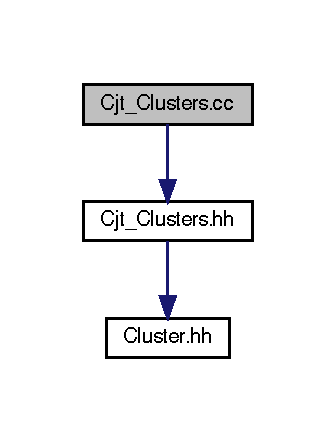
\includegraphics[width=161pt]{_cjt___clusters_8cc__incl}
\end{center}
\end{figure}


\subsection{Descripción detallada}
Implementación de la clase \hyperlink{class_cjt___clusters}{Cjt\+\_\+\+Clusters}. 


\hypertarget{_cjt___clusters_8hh}{}\section{Referencia del Archivo Cjt\+\_\+\+Clusters.\+hh}
\label{_cjt___clusters_8hh}\index{Cjt\+\_\+\+Clusters.\+hh@{Cjt\+\_\+\+Clusters.\+hh}}


Especificación \hyperlink{class_cjt___clusters}{Cjt\+\_\+\+Clusters}.  


Dependencia gráfica adjunta para Cjt\+\_\+\+Clusters.\+hh\+:
\nopagebreak
\begin{figure}[H]
\begin{center}
\leavevmode
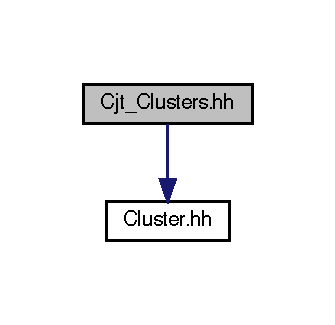
\includegraphics[width=161pt]{_cjt___clusters_8hh__incl}
\end{center}
\end{figure}
\subsection*{Clases}
\begin{DoxyCompactItemize}
\item 
class \hyperlink{class_cjt___clusters}{Cjt\+\_\+\+Clusters}
\begin{DoxyCompactList}\small\item\em Representa el ciclo evolutivo de los clusters según la diferencia de distancias entre estos. \end{DoxyCompactList}\end{DoxyCompactItemize}
\subsection*{defines}
\begin{DoxyCompactItemize}
\item 
\#define \hyperlink{_cjt___clusters_8hh_a1a1fe71433995a3b24bda7fea6e55fb1}{\+\_\+\+C\+J\+T\+\_\+\+E\+S\+P\+E\+C\+I\+E\+S\+\_\+\+H\+H\+\_\+}
\end{DoxyCompactItemize}


\subsection{Descripción detallada}
Especificación \hyperlink{class_cjt___clusters}{Cjt\+\_\+\+Clusters}. 



\subsection{Documentación de los \textquotesingle{}defines\textquotesingle{}}
\mbox{\Hypertarget{_cjt___clusters_8hh_a1a1fe71433995a3b24bda7fea6e55fb1}\label{_cjt___clusters_8hh_a1a1fe71433995a3b24bda7fea6e55fb1}} 
\index{Cjt\+\_\+\+Clusters.\+hh@{Cjt\+\_\+\+Clusters.\+hh}!\+\_\+\+C\+J\+T\+\_\+\+E\+S\+P\+E\+C\+I\+E\+S\+\_\+\+H\+H\+\_\+@{\+\_\+\+C\+J\+T\+\_\+\+E\+S\+P\+E\+C\+I\+E\+S\+\_\+\+H\+H\+\_\+}}
\index{\+\_\+\+C\+J\+T\+\_\+\+E\+S\+P\+E\+C\+I\+E\+S\+\_\+\+H\+H\+\_\+@{\+\_\+\+C\+J\+T\+\_\+\+E\+S\+P\+E\+C\+I\+E\+S\+\_\+\+H\+H\+\_\+}!Cjt\+\_\+\+Clusters.\+hh@{Cjt\+\_\+\+Clusters.\+hh}}
\subsubsection{\texorpdfstring{\+\_\+\+C\+J\+T\+\_\+\+E\+S\+P\+E\+C\+I\+E\+S\+\_\+\+H\+H\+\_\+}{\_CJT\_ESPECIES\_HH\_}}
{\footnotesize\ttfamily \#define \+\_\+\+C\+J\+T\+\_\+\+E\+S\+P\+E\+C\+I\+E\+S\+\_\+\+H\+H\+\_\+}



Definición en la línea 5 del archivo Cjt\+\_\+\+Clusters.\+hh.


\hypertarget{_cjt___especies_8cc}{}\section{Referencia del Archivo Cjt\+\_\+\+Especies.\+cc}
\label{_cjt___especies_8cc}\index{Cjt\+\_\+\+Especies.\+cc@{Cjt\+\_\+\+Especies.\+cc}}


Implementación de la clase \hyperlink{class_cjt___especies}{Cjt\+\_\+\+Especies}.  


Dependencia gráfica adjunta para Cjt\+\_\+\+Especies.\+cc\+:
\nopagebreak
\begin{figure}[H]
\begin{center}
\leavevmode
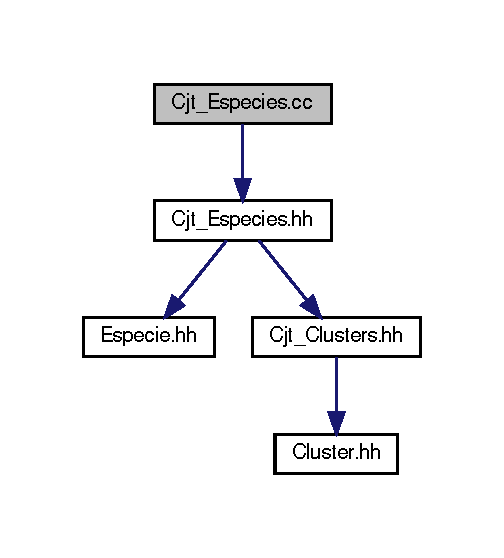
\includegraphics[width=242pt]{_cjt___especies_8cc__incl}
\end{center}
\end{figure}


\subsection{Descripción detallada}
Implementación de la clase \hyperlink{class_cjt___especies}{Cjt\+\_\+\+Especies}. 


\hypertarget{_cjt___especies_8hh}{}\section{Referencia del Archivo Cjt\+\_\+\+Especies.\+hh}
\label{_cjt___especies_8hh}\index{Cjt\+\_\+\+Especies.\+hh@{Cjt\+\_\+\+Especies.\+hh}}


Especificación \hyperlink{class_cjt___especies}{Cjt\+\_\+\+Especies}.  


Dependencia gráfica adjunta para Cjt\+\_\+\+Especies.\+hh\+:
\nopagebreak
\begin{figure}[H]
\begin{center}
\leavevmode
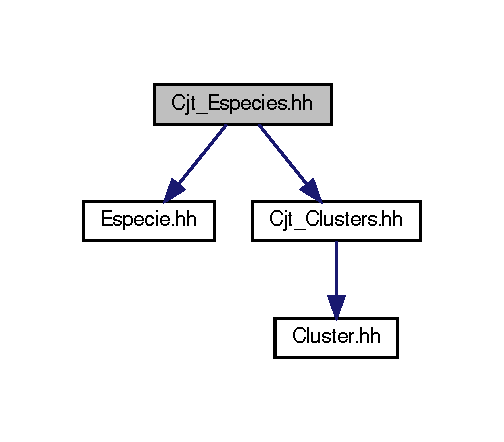
\includegraphics[width=242pt]{_cjt___especies_8hh__incl}
\end{center}
\end{figure}
\subsection*{Clases}
\begin{DoxyCompactItemize}
\item 
class \hyperlink{class_cjt___especies}{Cjt\+\_\+\+Especies}
\begin{DoxyCompactList}\small\item\em Representa la agrupación de las especies y una serie de operaciones para formar este conjunto. \end{DoxyCompactList}\end{DoxyCompactItemize}


\subsection{Descripción detallada}
Especificación \hyperlink{class_cjt___especies}{Cjt\+\_\+\+Especies}. 


\hypertarget{_cluster_8cc}{}\section{Referencia del Archivo Cluster.\+cc}
\label{_cluster_8cc}\index{Cluster.\+cc@{Cluster.\+cc}}


Implementación de la clase \hyperlink{class_cluster}{Cluster}.  


Dependencia gráfica adjunta para Cluster.\+cc\+:
\nopagebreak
\begin{figure}[H]
\begin{center}
\leavevmode
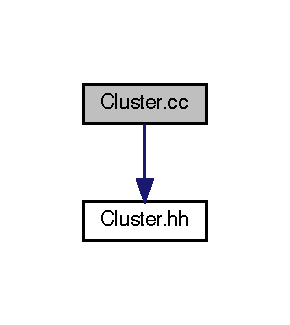
\includegraphics[width=139pt]{_cluster_8cc__incl}
\end{center}
\end{figure}


\subsection{Descripción detallada}
Implementación de la clase \hyperlink{class_cluster}{Cluster}. 


\hypertarget{_cluster_8hh}{}\section{Referencia del Archivo Cluster.\+hh}
\label{_cluster_8hh}\index{Cluster.\+hh@{Cluster.\+hh}}


Especificación de \hyperlink{class_cluster}{Cluster}.  


\subsection*{Clases}
\begin{DoxyCompactItemize}
\item 
class \hyperlink{class_cluster}{Cluster}
\begin{DoxyCompactList}\small\item\em Representa el conjunto de características y operaciones de los clústers. \end{DoxyCompactList}\end{DoxyCompactItemize}


\subsection{Descripción detallada}
Especificación de \hyperlink{class_cluster}{Cluster}. 


\hypertarget{_especie_8cc}{}\section{Referencia del Archivo Especie.\+cc}
\label{_especie_8cc}\index{Especie.\+cc@{Especie.\+cc}}


Implementación de la clase \hyperlink{class_especie}{Especie}.  


Dependencia gráfica adjunta para Especie.\+cc\+:
\nopagebreak
\begin{figure}[H]
\begin{center}
\leavevmode
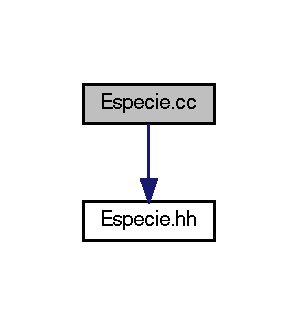
\includegraphics[width=143pt]{_especie_8cc__incl}
\end{center}
\end{figure}


\subsection{Descripción detallada}
Implementación de la clase \hyperlink{class_especie}{Especie}. 


\hypertarget{_especie_8hh}{}\section{Referencia del Archivo Especie.\+hh}
\label{_especie_8hh}\index{Especie.\+hh@{Especie.\+hh}}


Especificación de una classe \hyperlink{class_especie}{Especie}.  


\subsection*{Clases}
\begin{DoxyCompactItemize}
\item 
class \hyperlink{class_especie}{Especie}
\begin{DoxyCompactList}\small\item\em Representa el conjunto de características y operaciones de las especies. \end{DoxyCompactList}\end{DoxyCompactItemize}


\subsection{Descripción detallada}
Especificación de una classe \hyperlink{class_especie}{Especie}. 


\hypertarget{program_8cc}{}\section{Referencia del Archivo program.\+cc}
\label{program_8cc}\index{program.\+cc@{program.\+cc}}


Programa principal para el ejercicio {\itshape Evolución de las Especies}.  


Dependencia gráfica adjunta para program.\+cc\+:
\nopagebreak
\begin{figure}[H]
\begin{center}
\leavevmode
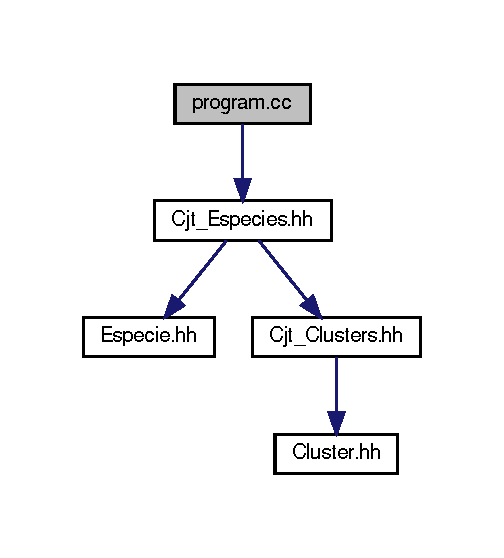
\includegraphics[width=242pt]{program_8cc__incl}
\end{center}
\end{figure}
\subsection*{Funciones}
\begin{DoxyCompactItemize}
\item 
int \hyperlink{program_8cc_ae66f6b31b5ad750f1fe042a706a4e3d4}{main} ()
\end{DoxyCompactItemize}


\subsection{Descripción detallada}
Programa principal para el ejercicio {\itshape Evolución de las Especies}. 

Los datos leídos determinan la operación que quiere ejecutar el usuario. Como estos datos de operación son del tipo string, el usuario seleccionará la operación introduciendo una string dentro de las disponibles. Dependiendo de la operación se necesitarán unos datos u otros. 

\subsection{Documentación de las funciones}
\mbox{\Hypertarget{program_8cc_ae66f6b31b5ad750f1fe042a706a4e3d4}\label{program_8cc_ae66f6b31b5ad750f1fe042a706a4e3d4}} 
\index{program.\+cc@{program.\+cc}!main@{main}}
\index{main@{main}!program.\+cc@{program.\+cc}}
\subsubsection{\texorpdfstring{main()}{main()}}
{\footnotesize\ttfamily int main (\begin{DoxyParamCaption}{ }\end{DoxyParamCaption})}



Definición en la línea 25 del archivo program.\+cc.


\begin{DoxyCode}
25            \{
26 
27   \hyperlink{class_cjt___especies}{Cjt\_Especies} cjt\_esp;
28   \hyperlink{class_cjt___clusters}{Cjt\_Clusters} clusts;
29 
30   \textcolor{keywordtype}{string} op; \textcolor{comment}{//código de operación}
31   \textcolor{keywordtype}{int} nesp; \textcolor{comment}{//número de especies}
32   \textcolor{keywordtype}{int} k;  \textcolor{comment}{//tamaño de subcadenas de gen}
33 
34   cin >> k;
35 
36   \textcolor{keywordtype}{string} ident, gen; \textcolor{comment}{//identidad y gen}
37 
38   cin >> op;
39   \textcolor{keywordflow}{while} (op != \textcolor{stringliteral}{"fin"})\{
40 
41     \textcolor{keywordflow}{if} (op == \textcolor{stringliteral}{"crea\_especie"})\{
42         cout << \textcolor{charliteral}{'#'} << \textcolor{charliteral}{' '} << op ;      
43         cin >> ident >> gen ;
44         cout << \textcolor{charliteral}{' '} << ident << \textcolor{charliteral}{' '} << gen << endl;
45 
46         \textcolor{keywordflow}{if} (not cjt\_esp.\hyperlink{class_cjt___especies_a7500b2ef69fc99e66948ee4e34e60fb2}{existe\_especie}(ident))\{
47             cjt\_esp.\hyperlink{class_cjt___especies_a94019f4a9bb2117abf8d0d1aa507fe2e}{crea\_especie}(ident, gen, k);
48         \}
49         \textcolor{keywordflow}{else} cout << \textcolor{stringliteral}{"ERROR: La especie "} << ident << \textcolor{stringliteral}{" ya existe."} << endl;
50         cout << endl;
51     \}
52 
53     \textcolor{keywordflow}{else} \textcolor{keywordflow}{if} (op == \textcolor{stringliteral}{"obtener\_gen"})\{
54         cout << \textcolor{charliteral}{'#'} << \textcolor{charliteral}{' '} << op ;
55         cin >> ident;
56         cout << \textcolor{charliteral}{' '} << ident << endl;
57 
58         \textcolor{keywordflow}{if} (cjt\_esp.\hyperlink{class_cjt___especies_a7500b2ef69fc99e66948ee4e34e60fb2}{existe\_especie}(ident))\{
59             \textcolor{keywordtype}{string} gen\_aux;
60             gen\_aux = cjt\_esp.\hyperlink{class_cjt___especies_a4cc8f3f5c7f0eadbb19526bbc1ab10bc}{obtener\_gen}(ident);
61             cout << gen\_aux << endl;
62         \} 
63         \textcolor{keywordflow}{else} cout << \textcolor{stringliteral}{"ERROR: La especie "} << ident << \textcolor{stringliteral}{" no existe."} << endl;
64         cout << endl;
65     \}
66 
67     \textcolor{keywordflow}{else} \textcolor{keywordflow}{if} (op == \textcolor{stringliteral}{"distancia"}) \{
68       cout << \textcolor{charliteral}{'#'} << \textcolor{charliteral}{' '} << op << \textcolor{charliteral}{' '};
69       \textcolor{keywordtype}{string} ident2;
70       cin >> ident >> ident2;
71       cout << ident << \textcolor{charliteral}{' '} << ident2 << endl;
72       \textcolor{keywordflow}{if} (cjt\_esp.\hyperlink{class_cjt___especies_a7500b2ef69fc99e66948ee4e34e60fb2}{existe\_especie}(ident) and cjt\_esp.\hyperlink{class_cjt___especies_a7500b2ef69fc99e66948ee4e34e60fb2}{existe\_especie}(ident2)) \{
73           cout << cjt\_esp.\hyperlink{class_cjt___especies_a14c0282be94e2520cca51539118b5b76}{distancia}(ident, ident2) << endl;
74       \}
75       \textcolor{keywordflow}{else} \textcolor{keywordflow}{if} (cjt\_esp.\hyperlink{class_cjt___especies_a7500b2ef69fc99e66948ee4e34e60fb2}{existe\_especie}(ident) and not cjt\_esp.
      \hyperlink{class_cjt___especies_a7500b2ef69fc99e66948ee4e34e60fb2}{existe\_especie}(ident2)) \{
76           cout << \textcolor{stringliteral}{"ERROR: La especie "} << ident2 << \textcolor{stringliteral}{" no existe."} << endl;
77       \}
78       \textcolor{keywordflow}{else} \textcolor{keywordflow}{if} (not cjt\_esp.\hyperlink{class_cjt___especies_a7500b2ef69fc99e66948ee4e34e60fb2}{existe\_especie}(ident) and cjt\_esp.
      \hyperlink{class_cjt___especies_a7500b2ef69fc99e66948ee4e34e60fb2}{existe\_especie}(ident2)) \{
79           cout << \textcolor{stringliteral}{"ERROR: La especie "} << ident << \textcolor{stringliteral}{" no existe."} << endl;
80       \}
81       \textcolor{keywordflow}{else} \{
82           cout << \textcolor{stringliteral}{"ERROR: La especie "} << ident << \textcolor{stringliteral}{" y la especie "} << ident2 << \textcolor{stringliteral}{" no existen."} << endl;
83       \} 
84       cout << endl;
85     \}
86 
87     \textcolor{keywordflow}{else} \textcolor{keywordflow}{if} (op == \textcolor{stringliteral}{"elimina\_especie"})\{
88         cout << \textcolor{charliteral}{'#'} << \textcolor{charliteral}{' '} << op ;
89         cin >> ident;
90         cout << \textcolor{charliteral}{' '} << ident << endl;
91 
92         \textcolor{keywordflow}{if} (cjt\_esp.\hyperlink{class_cjt___especies_a7500b2ef69fc99e66948ee4e34e60fb2}{existe\_especie}(ident))\{
93             cjt\_esp.\hyperlink{class_cjt___especies_aefad42bebc96b7bc924053630b365fbd}{elimina\_especie}(ident);
94         \}
95         \textcolor{keywordflow}{else} cout << \textcolor{stringliteral}{"ERROR: La especie "} << ident << \textcolor{stringliteral}{" no existe."} << endl;
96         cout << endl;
97     \}
98 
99     \textcolor{keywordflow}{else} \textcolor{keywordflow}{if} (op == \textcolor{stringliteral}{"existe\_especie"})\{
100         cout << \textcolor{charliteral}{'#'} << \textcolor{charliteral}{' '} << op ;
101         cin >> ident;
102         cout << \textcolor{charliteral}{' '} << ident << endl;
103         \textcolor{keywordflow}{if} (cjt\_esp.\hyperlink{class_cjt___especies_a7500b2ef69fc99e66948ee4e34e60fb2}{existe\_especie}(ident)) cout << \textcolor{stringliteral}{"SI"} << endl;
104         \textcolor{keywordflow}{else} cout << \textcolor{stringliteral}{"NO"} << endl;
105         cout << endl;
106     \}
107 
108     \textcolor{keywordflow}{else} \textcolor{keywordflow}{if} (op == \textcolor{stringliteral}{"lee\_cjt\_especies"})\{
109         cin >> nesp;
110         cjt\_esp.\hyperlink{class_cjt___especies_a3550a8bb7970521eba6efa70afad88b4}{lee\_cjt\_especies}(nesp, k);
111         cout << \textcolor{charliteral}{'#'} << \textcolor{charliteral}{' '} << op << endl;
112         cout << endl;
113     \}
114 
115     \textcolor{keywordflow}{else} \textcolor{keywordflow}{if} (op == \textcolor{stringliteral}{"imprime\_cjt\_especies"})\{
116         cout << \textcolor{charliteral}{'#'} << \textcolor{charliteral}{' '} << op << endl;
117         cjt\_esp.\hyperlink{class_cjt___especies_a61b0168970e926d3a27faf3f31ad2869}{imprime\_cjt\_especies}();
118         cout << endl;
119     \}
120 
121     \textcolor{keywordflow}{else} \textcolor{keywordflow}{if} (op == \textcolor{stringliteral}{"tabla\_distancias"})\{
122         cout << \textcolor{charliteral}{'#'} << \textcolor{charliteral}{' '} << op << endl;
123         cjt\_esp.\hyperlink{class_cjt___especies_a539b1f0c4b31a868e5961dc9a6920497}{tabla\_distancias}();
124         cout << endl;
125     \}
126 
127     \textcolor{keywordflow}{else} \textcolor{keywordflow}{if} (op == \textcolor{stringliteral}{"inicializa\_clusters"})\{
128       cout << \textcolor{charliteral}{'#'} << \textcolor{charliteral}{' '} << op << endl;
129       cjt\_esp.\hyperlink{class_cjt___especies_ae599e4e30a1d77e435395b796f821e06}{inicializa\_clusters}(clusts);
130       clusts.\hyperlink{class_cjt___clusters_a3f56a11d83d14d8dc58df32ea70163fa}{imprime\_clust\_distancias}();
131       cout << endl;
132     \}
133 
134     \textcolor{keywordflow}{else} \textcolor{keywordflow}{if} (op == \textcolor{stringliteral}{"ejecuta\_paso\_wpgma"})\{
135       cout << \textcolor{charliteral}{'#'} << \textcolor{charliteral}{' '} << op << endl;
136       \textcolor{keywordflow}{if} (clusts.\hyperlink{class_cjt___clusters_adf61aa25dfe16d52c5453d048df5efff}{es\_posible}()) \{
137         clusts.\hyperlink{class_cjt___clusters_a74ce6f42cecc4c26fea5a6ea21fa4123}{ejecuta\_paso\_wpgma}();
138         clusts.\hyperlink{class_cjt___clusters_a3f56a11d83d14d8dc58df32ea70163fa}{imprime\_clust\_distancias}();
139       \}
140       \textcolor{keywordflow}{else} cout << \textcolor{stringliteral}{"ERROR: num\_clusters <= 1"} << endl;
141       cout << endl;
142     \}
143 
144     \textcolor{keywordflow}{else} \textcolor{keywordflow}{if} (op == \textcolor{stringliteral}{"imprime\_cluster"})\{
145       cin  >> ident;
146       cout << \textcolor{charliteral}{'#'} << \textcolor{charliteral}{' '} << op << \textcolor{charliteral}{' '} << ident << endl;
147       \textcolor{keywordflow}{if} (clusts.\hyperlink{class_cjt___clusters_a989a4f3092a2bd47dc9a855107aa5086}{existe\_cluster}(ident))\{
148         clusts.\hyperlink{class_cjt___clusters_a17f8056edf94da434c058b0a7758b93c}{imprime\_cluster}(ident);
149       \}
150       \textcolor{keywordflow}{else} cout << \textcolor{stringliteral}{"ERROR: El cluster "} << ident << \textcolor{stringliteral}{" no existe."} << endl;
151       cout << endl;
152     \}
153 
154     \textcolor{keywordflow}{else} \textcolor{keywordflow}{if} (op == \textcolor{stringliteral}{"imprime\_arbol\_filogenetico"}) \{
155       cout << \textcolor{charliteral}{'#'} <<\textcolor{charliteral}{' '} << op << endl;
156       cjt\_esp.\hyperlink{class_cjt___especies_ae599e4e30a1d77e435395b796f821e06}{inicializa\_clusters}(clusts);
157       \textcolor{keywordflow}{if} (not clusts.\hyperlink{class_cjt___clusters_aeeea0be1e59431ef029fb42ce1aaddc6}{vacio}()) \{
158         clusts.\hyperlink{class_cjt___clusters_a95262506a2fdc5455ce104fb84649ee9}{imprime\_arbol\_filogenetico}();
159         cout << endl;
160       \}
161       \textcolor{keywordflow}{else} \{
162         cout << \textcolor{stringliteral}{"ERROR: El conjunto de clusters es vacio."} << endl;
163       \}
164       cout << endl;
165     \}
166     cin >> op;
167   \}
168 \}
\end{DoxyCode}

%--- End generated contents ---

% Index
\backmatter
\newpage
\phantomsection
\clearemptydoublepage
\addcontentsline{toc}{chapter}{Índice}
\printindex

\end{document}
